\begin{figure}[!h]
    \centering
    \resizebox{0.87\textwidth}{!}{
        \begin{tikzpicture}[mindmap,
        level 1 concept/.append style={level distance=130,sibling angle=120},
        level 2/.append style={level distance=100,sibling angle=120},
        ]
        \path[mindmap,concept color=black,text=white]
        node[concept] {Function}
        [clockwise from=0]
        child[concept color=blue,sibling angle=0,text=black]{
          node[concept] (periodic) {Periodic\\Functions}
          [clockwise from=0]
          child[concept color=green!50!black,sibling angle=90] {
              node[concept] (trigFunctions) {Trig.\\Functions}
              [clockwise from=55]
              child[concept color=green!50!black,sibling angle=90] {
                node[concept] (tangent) {Tangent}
              }
              child[concept color=green!50!black,sibling angle=90] {
                node[concept] (sine) {Sine}
              }
              child[concept color=green!50!black,sibling angle=90] {
                node[concept] (cosine) {Cosine}
              }
          }
          child[concept color=blue,sibling angle=98,level distance=110,font=\fontsize{8pt}{10pt}\selectfont] {
            node[concept,scale=1.4] (oscillations) {Oscillations}
            [clockwise from=-90]
            child[concept color=blue,sibling angle=45,level distance=80,font=\fontsize{4pt}{6pt}\selectfont] {
              node[concept,scale=1.5] (frequency) {Frequency}
            }
            child[concept color=blue,sibling angle=45,level distance=80,font=\fontsize{4pt}{6pt}\selectfont] {
              node[concept,scale=1.5] (amplitude) {Amplitude}
            }
          }
        };

        \begin{pgfonlayer}{background}
%        \draw [color=blue,ultra thick,looseness=1.5,<-] (arcLength) [out=-22, in=-45] to (radians);
        \draw [left color=blue, right color=green!50!black, draw=white,
               decorate,decoration=circle connection bar]
               (oscillations.east) -- (sine.south);
        \draw [left color=blue, right color=green!50!black, draw=white,
               decorate,decoration=circle connection bar]
               (oscillations.east) -- (cosine.south);
%        \draw [color=blue,ultra thick,looseness=1.5,<-] (arcArea) [out=0, in=-45] to (radians);
        \end{pgfonlayer}


        \end{tikzpicture}
      }
      \caption{Topics for the section on trigonometric functions.}
\end{figure}

\preClass{Coordinate Systems}

\videoLink{Section 4.3}{https://www.youtube.com/playlist?list=PLYHZK3b8UFw2K5Q_epS1Wi1hezUGCYwtP}

\begin{enumerate}
\item  Find the exact values of the six trigonometric functions $\theta$ and $\alpha$.  Use the following triangle.


%\trigTriangle{$\theta$}{$\alpha$}{5}{}{2}

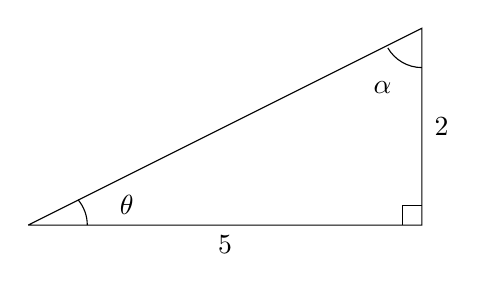
\begin{tikzpicture}[scale=2.5]
  \draw (0,0) -- (2,0) -- (2,1) -- (0,0);
  \draw (1.9,0) -- (1.9,0.1) -- (2,0.1);
  \draw (0.3,0) arc(0:40:0.2);
  \draw (0.5,0.1) node { $\theta$ };
  \draw (1.8,0.7) node { $\alpha$ };
  \draw (1,-0.1) node { 5 };
  \draw (1,0.6) node { ~ };
  \draw (2,0.8) arc(270:210:0.2);
  \draw (2.1,0.5) node { 2 };
\end{tikzpicture}


\begin{enumerate}
\begin{multicols}{2}
\item $\sin(\theta)=$\\[2.5em]
\item $\cos(\theta)=$\\[2.5em]
\item $\tan(\theta)=$\\[2.5em]
\item $\csc(\theta)=$\\[2.5em]
\item $\sec(\theta)=$\\[2.5em]
\item $\cot(\theta)=$\\[2.5em]

\columnbreak
\item $\sin(\alpha)=$\\[2.5em]
\item $\cos(\alpha)=$\\[2.5em]
\item $\tan(\alpha)=$\\[2.5em]
\item $\csc(\alpha)=$\\[2.5em]
\item $\sec(\alpha)=$\\[2.5em]
\item $\cot(\alpha)=$\\[2.5em]

\end{multicols}
\end{enumerate}

\clearpage

\item An observer at the top of a 462 ft mountain cliff measures the
  angle of depression from the top of the cliff to a point on the
  ground to be $5^\circ$.  What is the distance from the base (bottom)
  of the mountain to the point on the ground?  Round to the nearest
  foot. (Make a rough sketch of the situation clearly marking the
  relevant angles and distances before working out the problem.) If
  the angle of depression is a little bit bigger than $5^\circ$ will
  the distance increase or decrease? (Briefly justify your answer.)

  \vfill






\end{enumerate}






\actTitle{Worksheet 4.3}



\noindent \textbf{Instructions:}  Work together in groups of  3 or 4 to complete the following problems.\\

Student goals:
\begin{itemize}
\item Determine values of trigonometric functions given right triangles.
\item Use the Pythagorean identity to determine the value of one
  trigonometric function in terms of another.
\item Determine the values of trigonometric functions using multiple
  right triangles.
\item Translate a written description of a problem into a
  trigonometric formulation
\end{itemize}


\begin{enumerate}

\item Find the exact values of the six trigonometric functions of $\theta$ and $\alpha$
\begin{enumerate}
\item Use the following triangle.\\
\trigTriangle{$\theta$}{$\alpha$}{8}{10}{~}
\vfill

\item Use the following triangle.\\
\trigTriangle{$\theta$}{$\alpha$}{15}{~}{8}
\vfill
\end{enumerate}

\clearpage 

\item Use the isosceles right triangle and the 30/60/90 triangle to complete the table.

\begin{table}[h]
\begin{tabular}{|l|m{.12\textwidth}|m{.12\textwidth}|m{.12\textwidth}|m{.12\textwidth}|m{.12\textwidth}|m{.12\textwidth}|}
\hline
\textbf{$\theta$}        & \textbf{$\sin(\theta)$} & \textbf{$\cos(\theta)$} & \textbf{$\tan(\theta)$} & \textbf{$\csc(\theta)$} & \textbf{$\sec(\theta)$} & \textbf{$\cot(\theta)$} \\ \hline
30$^\circ=\frac{\pi}{6}$ &                         &                         &                         &                         &                         &                         \\  [2em] \hline
45$^\circ=\frac{\pi}{4}$ &                         &                         &                         &                         &                         &                         \\  [2em] \hline
60$^\circ=\frac{\pi}{3}$ &                         &                         &                         &                         &                         &                         \\  [2em] \hline
\end{tabular}
\end{table}

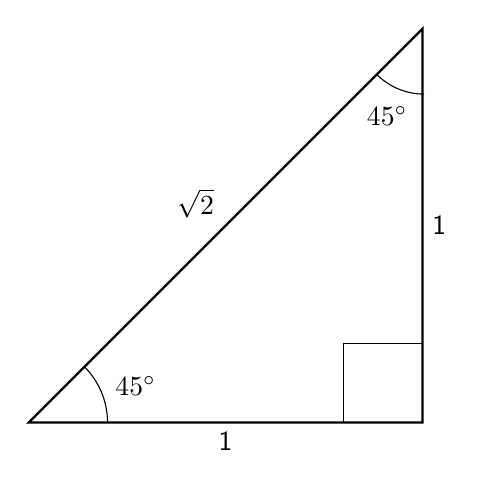
\begin{tikzpicture}[y=5cm, x=5cm,font=\sffamily]
  \draw[thick,black] (0,0) -- (1,0) -- (1,1) -- cycle;
  \draw[very thin,black] (0.8,0.0) -- (0.8,0.2) -- (1,0.2);
  \draw[thin,black] (0.2,0) arc (0:45:0.2);
  \node[black,anchor=north] at (0.5,0) {1};
  \node[black,anchor=west] at (1,0.5) {1};
  \node[black,anchor=south east] at (45:0.7) {$\sqrt{2}$};
  \node[black,anchor=south west] at (12.5:0.2) {$45^\circ$};
  \draw[thin,black] (45:1.25) arc (225:270:0.17);
  \node[black,anchor=west,xshift={8pt}] at (45:1.1) {$45^\circ$};
\end{tikzpicture}

\begin{tikzpicture}[y=5cm, x=5cm,font=\sffamily]
  \draw[thick,black] (0,0) -- (1,0) -- (60:2) -- cycle;
  \draw[thick,black,dashed] (1,0) -- (2,0) -- (60:2);
  \draw[very thin,black] (0.8,0.0) -- (0.8,0.2) -- (1,0.2);
  \draw[thin,black] (0.2,0) arc (0:60:0.2);
  \node[black,anchor=north] at (0.5,0) {1};
  \node[black,anchor=north] at (1.5,0) {1};
  \node[black,anchor=west] at (1,0.8) {$h$};
  \node[black,anchor=south east] at (60:1) {$2$};
  \node[black,anchor=south west] at (30:1.75) {$2$};
  \node[black,anchor=south west] at (12.5:0.2) {$60^\circ$};
  \draw[thin,black] (60:1.8) arc (240:270:0.2);
  \node[black,anchor=west] at (60:1.65) {$30^\circ$};
  \draw[thin,black] (1.8,0) arc (180:120:0.2) node[pos=0.5,anchor=south east] {$60^\circ$};
  \draw[thin,black] (1,1.535) arc (270:300:0.2) node[pos=0.,anchor=north west,yshift=-7] {$30^\circ$};
\end{tikzpicture}

\vfill

%\item
%\begin{enumerate}
%\item Evaluate $\sin(60^\circ)$.\\[0.2in]
%\item Evaluate $\sin(30^\circ)+\sin(30^\circ)$.\\[0.2in]
%\item Are the values in parts $(a)$ and $(b)$ the same?
%\end{enumerate}

\clearpage




\item For each problem below determine the values of the missing
  quantities. All angles are in radians, and your answers for angles
  should be in radians. (The triangles are not drawn to scale.)
\begin{enumerate}

\item ~ \\
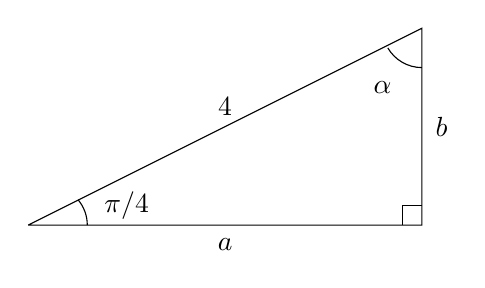
\begin{tikzpicture}[scale=2.5]
  \draw (0,0) -- (2,0) -- (2,1) -- (0,0);
  \draw (1.9,0) -- (1.9,0.1) -- (2,0.1);
  \draw (0.3,0) arc(0:40:0.2);
  \draw (0.5,0.1) node { $\pi/4$ };
  \draw (1.8,0.7) node { $\alpha$ };
  \draw (1,-0.1) node { $a$ };
  \draw (1,0.6) node { 4 };
  \draw (2,0.8) arc(270:210:0.2);
  \draw (2.1,0.5) node { $b$ };
\end{tikzpicture}
	
\framebox[0.3\textwidth][l]{
  \begin{tabular}{lc}
    $a$ & $=$ \\ [15pt]
    $b$ & $=$ \\ [15pt]
    $\alpha$ & $=$ \\
  \end{tabular}
}

\vfill

\item ~ \\
  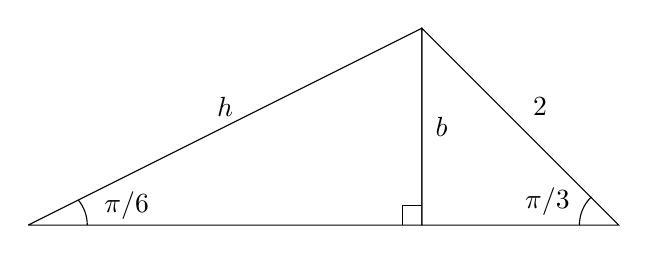
\begin{tikzpicture}[scale=2.5]
    \draw (0,0) -- (2,0) -- (2,1) -- (0,0);
    \draw (1.9,0) -- (1.9,0.1) -- (2,0.1);
    \draw (0.3,0) arc(0:40:0.2);
    \draw (0.5,0.1) node { $\pi/6$ };
    \draw (1,0.6) node { $h$ };
    \draw (2.1,0.5) node { $b$ };
    \draw (2,0) -- (3,0) -- (2,1) -- (2,0);
    \draw (2.8,0) arc(180:134:0.2);
    \draw (2.8,0) node[anchor=south east] { $\pi/3$ };
    \draw (2.6,0.6) node { $2$ };
  \end{tikzpicture}

	
  \framebox[0.3\textwidth][l]{
    \begin{tabular}{lc}
      $h$ & $=$ \\ [15pt]
      $b$ & $=$ \\ [15pt]
    \end{tabular}
  }
  
  \vfill

\end{enumerate}
\clearpage

\item A 30 ft boat ramp makes a $7^\circ$ angle with the water.  What
  is the height of the ramp above the water at the ramp's highest
  point?  Round to the nearest tenth of a foot.

  \vfill


\item At a tree farm, palm trees are harvested once they reach a
  height of 20 feet.  Suppose a farm worker determine's that the
  distance along the ground from her position to the base of a palm
  tree is 22 feet.  She then uses an instrument called a clinometer
  held at her eye level of 6 feet to measure the angle of elevation
  tot he top of the tree as $30.2^\circ$.  Is the tree tall enough to
  harvest?

  \vfill

  \clearpage

\item Robert Stroud is standing on top of a building, and he sees a
  pigeon on the ground away from the building. Robert’s angle of
  depression is $8.5^\circ$ as he stares at the bird. The bird hops
  15m directly away from the building, and the new angle of depression
  is $7.0^\circ$ .  What is the height of the building?


  \vfill

\end{enumerate}

\hwTitle{Section 4.3}

\begin{enumerate}
\item For each diagram below determine the values of the requested
  quantities.  All angles are in radians. (Figures are not drawn to
  scale.)

  \begin{enumerate}
    \item ~ \\

    \begin{minipage}[h]{0.4\linewidth}
      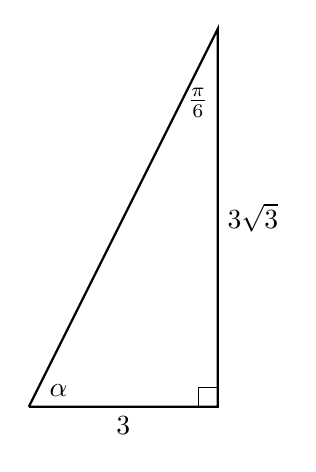
\begin{tikzpicture}[y=1.2cm, x=1.2cm,font=\sffamily]
        %% Draw the base, upright and hypotenuse
        \draw[thick] (0,0) -- (2,0) -- (2,4) -- (0,0); 
        \draw[thin] (0.9*2,0) -- (0.9*2,0.1*2) -- (2,0.1*2);
        \node[anchor=north] at (2/2,0) {$3$}; 
        \node[anchor=west] at (2,4/2) {$3\sqrt{3}$}; 
        %\node[anchor=south east] at (2/2,4/2) {$$};
        \node[anchor=south west,xshift=4] at (0,0) {$\alpha$};
        \node[anchor=north east,yshift=-18] at (2,4) {$\frac{\pi}{6}$};
      \end{tikzpicture}
    \end{minipage}
    \begin{minipage}[h]{0.4\linewidth}
      \begin{eqnarray*}
        \alpha & = & \\ [10pt]
        \sin(\alpha) & = & \\ [10pt]
        \tan(\alpha) & = & \\ [10pt]
      \end{eqnarray*}
    \end{minipage}

    \item ~ \\

    \begin{minipage}[h]{0.4\linewidth}
      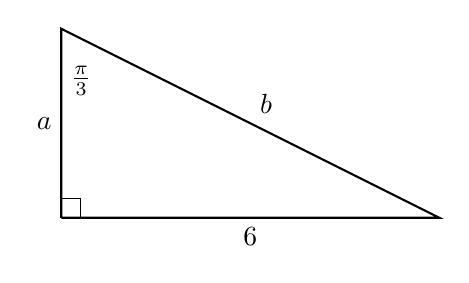
\begin{tikzpicture}[y=1.2cm, x=1.2cm,font=\sffamily]
        %% Draw the base, upright and hypotenuse
        \draw[thick] (0,0) -- (4,0) -- (0,2) -- (0,0); 
        \draw[thin] (0,0.1*2) -- (0.1*2,0.1*2) -- (0.1*2,0);
        \node[anchor=north] at (4/2,0) {$6$}; 
        \node[anchor=east] at (0,2/2) {$a$}; 
        \node[anchor=south west] at (4/2,2/2) {$b$};
        \node[anchor=south east,xshift=-24] at (4,0) {$$};
        \node[anchor=north west,yshift=-10] at (0,2) {$\frac{\pi}{3}$};
      \end{tikzpicture}
    \end{minipage}
    \begin{minipage}[h]{0.4\linewidth}
      \begin{eqnarray*}
        a & = & \\ [10pt]
        b & = & \\ [10pt]
      \end{eqnarray*}
    \end{minipage}

  \item ~ \\

    \begin{minipage}[h]{0.4\linewidth}
      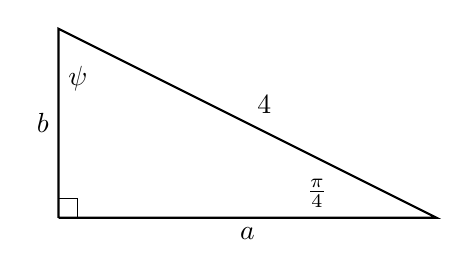
\begin{tikzpicture}[y=1.2cm, x=1.2cm,font=\sffamily]
        %% Draw the base, upright and hypotenuse
        \draw[thick] (0,0) -- (4,0) -- (0,2) -- (0,0); 
        \draw[thin] (0,0.1*2) -- (0.1*2,0.1*2) -- (0.1*2,0);
        \node[anchor=north] at (4/2,0) {$a$}; 
        \node[anchor=east] at (0,2/2) {$b$}; 
        \node[anchor=south west] at (4/2,2/2) {$4$};
        \node[anchor=south east,xshift=-36] at (4,0) {$\frac{\pi}{4}$};
        \node[anchor=north west,yshift=-10] at (0,2) {$\psi$};
      \end{tikzpicture}
    \end{minipage}
    \begin{minipage}[h]{0.4\linewidth}
      \begin{eqnarray*}
        a & = & \\ [10pt]
        b & = & \\ [10pt]
        \psi & = & \\ [10pt]
      \end{eqnarray*}
    \end{minipage}


    \item ~ \\

    \begin{minipage}[h]{0.4\linewidth}
      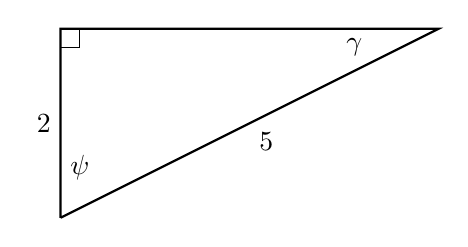
\begin{tikzpicture}[y=1.2cm, x=1.2cm,font=\sffamily]
        %% Draw the base, upright and hypotenuse
        \draw[thick] (0,0) -- (0,2) -- (4,2) -- (0,0); 
        \draw[thin] (0,0.9*2) -- (0.1*2,0.9*2) -- (0.1*2,2);
        %\node[anchor=south] at (4/2,2) {$a$}; 
        \node[anchor=east] at (0,2/2) {$2$}; 
        \node[anchor=north west] at (4/2,2/2) {$5$};
        \node[anchor=north east,xshift=-24] at (4,2) {$\gamma$};
        \node[anchor=south west,yshift=10] at (0,0) {$\psi$};
      \end{tikzpicture}
    \end{minipage} 
    \begin{minipage}[h]{0.4\linewidth}
      \begin{eqnarray*}
        \cos(\psi) & = & \\ [10pt]
        \sin(\psi) & = & \\ [10pt]
        \tan(\gamma) & = & \\ [10pt]
      \end{eqnarray*}
    \end{minipage}
    

  \end{enumerate}

\item If a 15 ft ladder is leaning against a wall at an angle of
  $62^\circ$ with the ground, how high up the will the ladder reach?
  Round to the nearest tenth of a foot.


\item Two observers are standing a distance of 100m apart. They both
  spot an eagle and watch it closely. The moment it passes between
  them, the first observer measures an angle of elevation from the
  ground of $45^\circ$ , and the second observer measures an angle of
  elevation from the ground of $35^\circ$ . How high in the air was
  the eagle when it passed between the two observers?

\item Prince Henry stands on the balcony of his castle that faces the
  sea. The base of the castle is 100m West of the beach, and the
  balcony is 30m above sea level. The Prince's true love, the commoner
  Matilda, is cleaning fish on a ship that is 200m directly East of
  the beach in a direct line East of the Prince's balcony. At that
  instant, as the Prince gazes upon his true love's ship, what is the
  angle of depression of his crying eyes?

\item Determine the exact value of $\sin(\omega)$.
  
    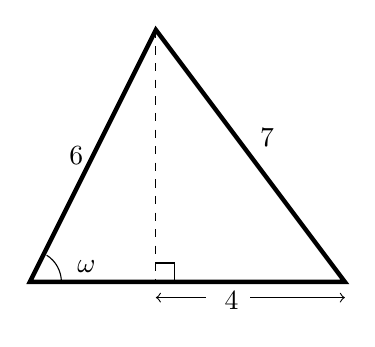
\begin{tikzpicture}[y=0.8cm, x=0.8cm,font=\sffamily]
      \draw[ultra thick,black] (0,0) -- (5,0) -- (2,4) -- cycle;
      \draw[black,dashed] (2,4) -- (2,0);
      \draw[black] (2,0.3) -- (2.3,0.3) -- (2.3,0);
      \node[anchor = south east] at (1.2,0)   {$\omega$};
      \node[anchor = east] at (1,2)         {$6$};
      \node[anchor = south west] at (3.5,2) {$7$};
      \node[anchor=north] at (3.2,0) {$4$};
      \draw[<-] (2,-0.25) -- (2.8,-0.25);
      \draw[->] (3.5,-0.25) -- (5,-0.25);
      \draw[black,thin] (0.5,0) arc (0:58:0.5);
    \end{tikzpicture}

\item Determine the exact value of $p$ in the figure below.

    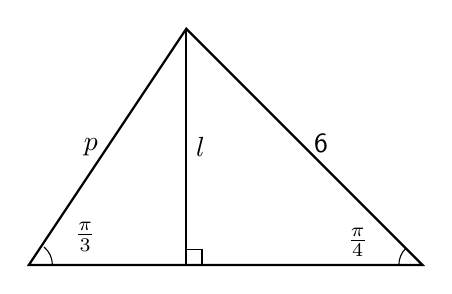
\begin{tikzpicture}[y=1.0cm, x=1.0cm,font=\sffamily]
      \draw[thick,black] (0,0) -- (2,3) -- (5,0) -- cycle;
      \draw[thick,black] (2,3) -- (2,0);
      \draw[thin,black] (2,0.2) -- (2.2,0.2) -- (2.2,0);
      \draw[thin,black] (4.7,0) arc (180:135:0.3);
      \draw[thin,black] (0.3,0) arc (0:50:0.3);
      \node[black,xshift=-23.4,yshift=8.2] at (5,0) {$\frac{\pi}{4}$};
      \node[black,xshift=20.4,yshift=10.2] at (0,0) {$\frac{\pi}{3}$};
      \node[black,anchor=south west] at (3.5,1.3) {6};
      \node[black,anchor=west] at (2,1.5) {$l$};
      \node[black,anchor=east] at (1,1.5) {$p$};
    \end{tikzpicture}


\item The area of a triangle is one half the length of its
  base multiplied by its height. Determine the area of the triangle
  shown below. \\ 
  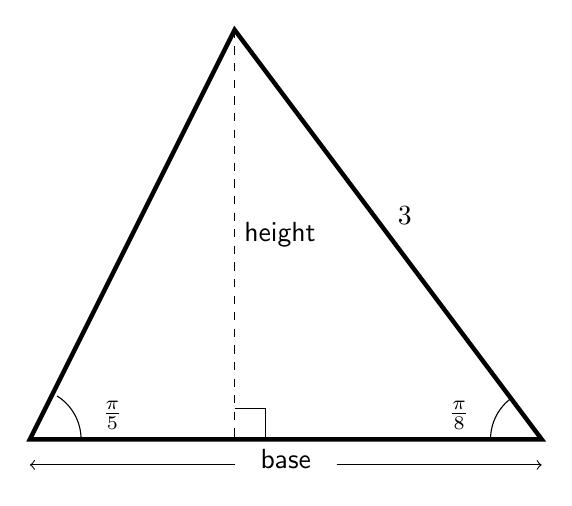
\begin{tikzpicture}[y=1.3cm, x=1.3cm,font=\sffamily]
    \draw[ultra thick,black] (0,0) -- (5,0) -- (2,4) -- cycle;
    \draw[black,dashed] (2,4) -- (2,0);
    \draw[black] (2,0.3) -- (2.3,0.3) -- (2.3,0);
    \node[anchor = south east] at (1.0,0)   {$\frac{\pi}{5}$};
    \node[anchor = south west] at (4.0,0)   {$\frac{\pi}{8}$};
    \node[anchor = south west] at (3.5,2) {$3$};
    \node[anchor = west] at (2,2) {height};
    \node[anchor=north] at (2.5,0) {base};
    \draw[<-] (0,-0.25) -- (2.,-0.25);
    \draw[->] (3,-0.25) -- (5,-0.25);
    \draw[black,thin] (0.5,0) arc (0:58:0.5);
    \draw[black,thin] (4.5,0) arc (180:125:0.5);
  \end{tikzpicture}

\item A person is standing forty meters from the base of a building,
  and the person is looking directly at a point halfway to the top of
  the building. The angle of elevation is $32^\circ$.  What will the
  angle of elevation be when the person is looking at the top of the
  building?

\item Sir Edmund Hillary is standing between two peaks, Mount Dampier
  and Mount Vancouver.  It is estimated that the two peaks are the
  same height. Sir Hillary is standing in a line directly between the
  two peaks, and he estimates that his distance to a point directly
  below the peak of Mount Dampier at his same altitude is seven
  hundred meters more than the distance to the equivalent point below
  Mount Vancouver. When looking at Mount Dampier he estimates the
  angle of elevation is $41.6^\circ$, and his angle of elevation for
  Mount Vancouver is $69.4^\circ$. What is the elevation of the two
  peaks above Sir Hillary's current elevation?

\end{enumerate}



  


\preClass{Coordinate Systems}


\videoLink{Section 4.4}{https://www.youtube.com/playlist?list=PLYHZK3b8UFw2OmnPlWMPeyRScOjE2Rk4C}


\begin{enumerate}
\item  Let $P(-2,-5)$ be a point on the terminal side of $\theta$.  Find each of the six trig functions of $\theta$.

\begin{enumerate}
\begin{multicols}{2}
\item $\sin(\theta)=$\\[.3in]
\item $\cos(\theta)=$\\[.3in]
\item $\tan(\theta)=$\\[.3in]
\columnbreak
\item $\csc(\theta)=$\\[.3in]
\item $\sec(\theta)=$\\[.3in]
\item $\cot(\theta)=$\\[.3in]







\end{multicols}
\end{enumerate}

\vfill
\item Label the side lengths of the given reference triangles.\\
\newcommand{\trigTriangle}[5]{%
	\begin{tikzpicture}[scale=2.5]
	\draw (0,0) -- (2,0) -- (2,1) -- (0,0);
	\draw (1.9,0) -- (1.9,0.1) -- (2,0.1);
	\draw (0.3,0) arc(0:40:0.2);
	\draw (0.5,0.1) node { #1 };
	\draw (1.8,0.7) node { #2 };
	\draw (1,-0.1) node { #3 };
	\draw (1,0.6) node { #4 };
	\draw (2,0.8) arc(270:210:0.2);
	\draw (2.1,0.5) node { #5 };
	\end{tikzpicture}
}
\begin{multicols}{2}
	\trigTriangle{$\frac{\pi}{6}$}{$\frac{\pi}{3}$}{}{}{} \quad \quad \quad \quad \quad \quad 
	\columnbreak
	\trigTriangle{$\frac{\pi}{4}$}{$\frac{\pi}{4}$}{}{ }{}

\end{multicols}
\clearpage


\item  Let $\displaystyle \theta=\frac{8\pi}{3}$.
\begin{enumerate}
\item Determine the reference angle $\theta_R$ for $\displaystyle \theta=\frac{8\pi}{3}$.\vfill
\item Determine $\sin\left(\frac{8\pi}{3}\right)$.\vfill
\item Determine $\cos\left(\frac{8\pi}{3}\right)$.\vfill
\end{enumerate}





\end{enumerate}






\actTitle{Worksheet 4.4}


\noindent \textbf{Instructions:}  Work together in groups of  3 or 4 to complete the following problems.\\
\noindent \textbf{NOTE:  Do not use your unit circle to answer the following questions.  Only use reference triangles.}

Student goals:
\begin{itemize}
\item Determine subsets of the domain where sine/cosine are increasing
  and where they are decreasing.
\item Determine whether a trigonometric function will increase or
  decrease given a specific angle.
\item Determine the reference angle of a given angle in any of the
  four quadrants.
\end{itemize}


\begin{enumerate}

\item Let $P(-7,\frac{\sqrt{3}}{4})$ be a point on the terminal side of $\theta$.  Find each of the six trig functions of $\theta$.\begin{enumerate}
\begin{multicols}{2}
\item $\sin(\theta)=$\\[1em]
\item $\cos(\theta)=$\\[1em]
\item $\tan(\theta)=$\\[1em]
\columnbreak
\item $\csc(\theta)=$\\[1em]
\item $\sec(\theta)=$\\[1em]
\item $\cot(\theta)=$\\[1em]
\end{multicols}
\end{enumerate}
\vfill

\item For each of the following questions $\theta$ is in standard
  position and  $\theta=2\pi/3$.
\begin{enumerate}
\item  What quadrant is $\theta$ in?
  \vfill
\item Determine the reference angle for $\theta$.
  \vfill
\item Determine exact values of each of the following and determine if
  the function is increasing, decreasing, or neither at $\theta$.
  % quadrant ii 
  \begin{enumerate}
  \item $\sin\left(\frac{2\pi}{3}\right)$
    \vfill
  \item $\cos\left(\frac{2\pi}{3}\right)$
    \vfill
  \item $\tan\left(\frac{2\pi}{3}\right)$
    \vfill
  \end{enumerate}

\end{enumerate}

\clearpage
\item For each of the following expressions, $t=\frac{7\pi}{2}$. For
  each expression determine the value and determine if the function is
  increasing, decreasing, or neither at $t$.
\begin{enumerate}
\item $\sin(t)$ \vfill
\item $\tan(t)$ \vfill
\item $\sec(t)$ \vfill
\end{enumerate}


\item In each question below  $\theta$ is an angle in standard
  position and  $\theta=\frac{16\pi}{3}$. 
  \begin{enumerate}
  \item What quadrant is $\theta$ in?  Determine the reference angle
    for $\theta$.
    \vfill
    \vfill

  \item Determine the exact values of $\sin(\theta)$, $\sec(\theta)$,
    and $\cot(\theta)$. For each value indicate if the function is
    increase, decreasing, or neither for this value of $\theta$.
    \vfill \vfill \vfill \vfill
\end{enumerate}
%\\[3in]

\clearpage
%QII 
\item \begin{enumerate}
  \item If $\theta$ is an angle in standard position, determine the
    quadrant corresponding to $\theta=-210^\circ$. Then determine the
    reference angle for $\theta=-210^\circ$.

    \vfill

  \item Determine the exact values of $\cos(\theta),$ $\csc(\theta)$,
    and $\tan(\theta)$ for $\theta=-210^\circ$.

    \vfill
    
\end{enumerate}








\item Suppose $\theta$ is an angle in the third quadrant with
  reference angle $\theta_R$ satisfying $\cos(\theta_R)=\frac{5}{13}$
  and $\sin(\theta_R)=\frac{12}{13}$.  Determine the exact values of
  $\cos(\theta)$ and $\csc(\theta)$.

  \vfill
  \vfill
  \vfill

\item An angle is in the second quadrant, and its reference angle is
  $\theta_R=\frac{2\pi}{9}$. Determine the radian measure of the
  angle.

  \vfill

\end{enumerate}



\hwTitle{Section 4.4}

\begin{enumerate}
\item  Determine exact values of the following.
  \begin{enumerate}
  \item $\sec\left(\frac{2\pi}{3}\right)$
  \item $\csc\left(\frac{2\pi}{3}\right)$
  \item $\cot\left(\frac{2\pi}{3}\right)$
  \end{enumerate}
\item Determine the following.
  \begin{enumerate}
  \item $\cos\left(\frac{7\pi}{2}\right)$
  \item $\csc\left(\frac{7\pi}{2}\right)$
  \item $\cot\left(\frac{7\pi}{2}\right)$
  \end{enumerate}
\item Determine the exact value of each of the following. %same ref
  \begin{enumerate}
  \item $\sin\left(\frac{7\pi}{6}\right)$ 
  \item $\sin\left(\frac{11\pi}{6}\right)$
  \item $\sin\left(\frac{5\pi}{6}\right)$ 
  \end{enumerate}
\item Find the value of each expression.
  \begin{enumerate}
  \item $\sin\left(30^\circ\right)\cdot \cos\left(150^\circ\right)\cdot \sec\left(60^\circ\right)\cdot \csc\left(120^\circ\right)$
  \item $\cos^2\left(\frac{5\pi}{4}\right)-\sin^2\left(\frac{2\pi}{3}\right)$
  \item $\sin^2\left(\frac{11\pi}{6}\right)+\cos^2\left(\frac{4\pi}{3}\right)$
  \item $\displaystyle \frac{2\tan\left(\frac{11\pi}{6}\right)}{1-\tan^2\left(\frac{11\pi}{6}\right)}$
  \end{enumerate}
\item An angle is in the third quadrant, and its reference angle is
  $\theta_R=\frac{5\pi}{12}$. Determine the radian measure of the
  angle.
\item Determine the reference angle for $\theta=5.7$ radians.
\item A function, $\textrm{Ref}(\theta)$, is defined so that it
  returns the reference angle of the given function. Make a sketch of
  the function for $0\leq\theta < 2\pi$. Express the function as
  piecewise defined function. Is the function periodic? Is it even,
  odd, or neither?


\end{enumerate}




\actTitle{Worksheet 4.1-4.4 Review}

\noindent \textbf{Instructions:}  Work together in groups of  3 or 4 to complete the following problems.\\


\begin{enumerate}

\item Consider the angle $\displaystyle \theta=\frac{7\pi}{4}$ which
  is in standard position.
\begin{enumerate}
\item  Draw a picture labeling $\displaystyle \theta=\frac{7\pi}{4}$
  and it's corresponding reference angle.
  
  \begin{tikzpicture}
    \draw[->,ultra thick] (-5,0)--(5,0) node[right]{$x$};
    \draw[->,ultra thick] (0,-5)--(0,5) node[above]{$y$};
  \end{tikzpicture}

\item Determine the reference angle.
  \vfill

\item Determine $\displaystyle \tan\left(\frac{7\pi}{4}\right)$.
  \vfill
  
\end{enumerate}


\clearpage

%\item Determine the angles, $\theta$, that match the criteria in each question below.
%\begin{enumerate}
%\item An angle that is coterminal with the angle $\alpha=\frac{\pi}{4}$ and is greater than $\pi$.\vfill
%\item An angle that is coterminal with the angle $\alpha=\frac{3\pi}{4}$ and is negative.\vfill
%\end{enumerate}

%\item An angle $\theta$ is in the second quadrant, and $\sin{\theta}=0.25$.  Determine the cosine of the angle.\vfill

\item An angle $\theta$ is in the fourth quadrant, and $\cos{\theta}=0.25$.  Determine the tangent of the angle.\vfill

\item Determine all the angles, $\theta$ between 0 and $3\pi$ such that $\cos{(\theta)}=-\frac{\sqrt{3}}{2}$.  Give exact answers in radians.\vfill




\item The terminal side of an angle $\theta$ in standard position goes
  through the point $(-6,-5).$  Find an exact answer for each of the following.
\begin{enumerate}
\item $\sin{(\theta)}$\vfill
\item $\cos{(\theta)}$\vfill
\item $\cot{(\theta)}$\vfill

\end{enumerate}

\clearpage

\item For each question below, a diagram of a point on a circle is
  given.  Answer each question about the angle formed by the line
  through the point, the origin, and the positive $x$-axis.
\begin{enumerate}
\item Determine the cosine of the angle $\theta$.  (Your answer should
  be a number and not have an $x$ in it.) \\
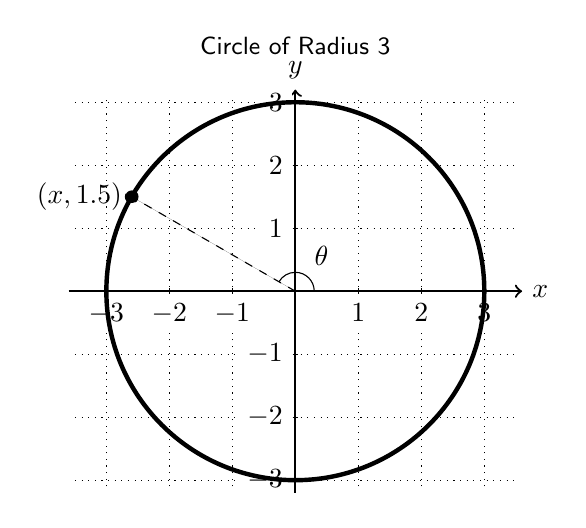
\begin{tikzpicture}[y=0.8cm, x=0.8cm,font=\sffamily]
  \draw[step=1,black, dotted] (-3.5,-3.1) grid (3.5,3.1); % very thin,
  \draw[thick,black,->] (-3.6,0) -- (3.6,0) node[anchor=west] {$x$};
  \draw[thick,black,->] (0,-3.2) -- (0,3.2) node[anchor=south] {$y$};
  \node[black] at (0,3.9) {\small Circle of Radius 3};

  \foreach \x in {-3,-2,-1,1,2,3} {
    \draw (\x,1pt) -- (\x,-1pt);
    \draw (\x,-1pt) node[anchor=north,fill=white] {$\x$};
  }

  \foreach \y in {-3,-2,-1,1,2,3}{
    \draw (-1pt,\y) -- (1pt,\y);
    \draw (-1pt,\y) node[anchor=east,fill=white] {$\y$};
  }

  \draw[ultra thick,black] (0,0) circle(3);
  \draw[black,dashed,fill=black] (0,0) -- (150:3) circle (0.1) node[anchor=east] {$(x,1.5)$};
  \node[black,anchor=south west] at (60:0.3)  {$\theta$};
  \draw[thin,black] (0:0.3) arc (0:150:0.3);
\end{tikzpicture}


\item Determine the tangent of the angle $\psi$.
  (Your answer should be a number and not have a $y$ in it.)\\
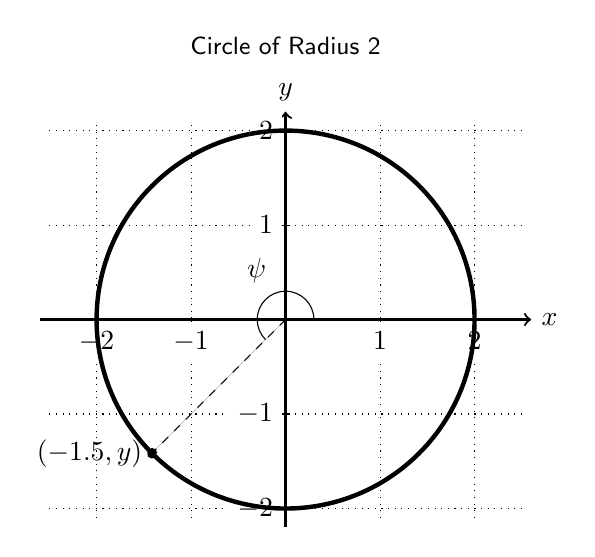
\begin{tikzpicture}[y=1.2cm, x=1.2cm,font=\sffamily]
  \draw[step=1,black, dotted] (-2.5,-2.1) grid (2.5,2.1); % very thin,
  \draw[thick,black,->] (-2.6,0) -- (2.6,0) node[anchor=west] {$x$};
  \draw[thick,black,->] (0,-2.2) -- (0,2.2) node[anchor=south] {$y$};
  \node[black] at (0,2.9) {\small Circle of Radius 2};

  \foreach \x in {-2,-1,1,2} {
    \draw (\x,1pt) -- (\x,-1pt);
    \draw (\x,-1pt) node[anchor=north,fill=white] {$\x$};
  }

  \foreach \y in {-2,-1,1,2}{
    \draw (-1pt,\y) -- (1pt,\y);
    \draw (-1pt,\y) node[anchor=east,fill=white] {$\y$};
  }

  \draw[ultra thick,black] (0,0) circle(2);
  \draw[black,dashed,fill=black] (0,0) -- (225:2) circle (0.05) node[anchor=east] {$(-1.5,y)$};
  \node[black,anchor=south east] at (110:0.3)  {$\psi$};
  \draw[thin,black] (0:0.3) arc (0:225:0.3);
\end{tikzpicture}

\end{enumerate}




\item Given the following, find the exact value of $\sin{(\alpha)}.$\\
  $$\cos{(\alpha)}=-\frac{1}{3} \quad
  \text{and}\quad \tan{(\alpha)} \quad \text{is negative}$$
  Which quadrants could the angle be in?
  \vfill

  \clearpage
  
\item A ship is anchored a distance of $d=150$m from a beach.  A
  spotlight on the bow of the ship can rotate, and the angle is
  measured from a line perpendicular to the beach that goes through
  the base of the spotlight.  Determine the position, $y$, along the
  beach that the spotlight will illuminate the given angle, $\theta$.
  (Your answer should be a function of $\theta$
  with $-\pi/2<\theta <\pi/2.)$\\
  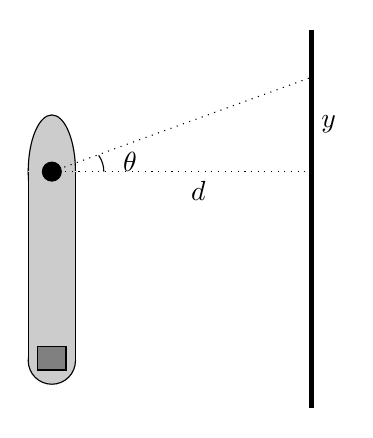
\begin{tikzpicture}[y=1.2cm, x=1.2cm,font=\sffamily]
    %\node[black] at (0,2.9) {\small Circle of Radius 2};

    %\draw[ultra thick,black] (0,0) circle(2);
    %\draw[black,dashed,fill=black] (0,0) -- (225:2) circle (0.05) node[anchor=east] {$(-1.5,y)$};
    %\node[black,anchor=south east] at (110:0.3)  {$\psi$};
    %\draw[thin,black] (0:0.3) arc (0:225:0.3);

    \filldraw[black!20] (0.25,0) circle (0.25);
    \filldraw[black!20] (0.25,2) ellipse (0.25 and 0.6);
    \draw[black] (0.25,2) ellipse (0.25 and 0.6);
    \draw[black] (0.25,0) circle (0.25);
    \filldraw[black!20] (0,0) rectangle(0.5,2);
    \draw[black,fill=black!50] (0.1,-0.1) rectangle(0.4,0.15);
    \draw[black] (0,0) -- (0,2);
    \draw[black] (0.5,0) -- (0.5,2);
    \filldraw[black] (0.25,2) circle(0.1);

    \draw[black,dotted] (0.25,2) -- (3,2);
    \draw[black,dotted] (0.25,2) -- (3,3);
    \draw[black,ultra thick] (3,-0.5) -- (3,3.5);
    \draw[black] (0.8,2) arc (0:35:0.3);

    \node[anchor=west] at (0.9,2.1) {$\theta$};
    \node[anchor=north] at (1.8,2) {$d$};
    \node[anchor=west] at (3,2.5) {$y$};
  \end{tikzpicture}

  

\item A surveyor wishes to determine the height of a building. The
  surveyor is standing directly in front of the building and measures
  an angle of elevation of $17^\circ$ to the top of the building. The
  surveyor then backs up ten meters and measures an angle of
  elevation of $14^\circ$. What is the height of the building?

  \vfill
  \vfill

\item A frog rides a unicycle that has a wheel with a diameter of 1.5
  inches.  If the frog travels a distance of 320 inches, what is the
  angle that the wheel turned?  Give an exact answer.

  \vfill


\clearpage


\item A pizza shop owner feels inspired after taking a precalculus class at his local college.  He decides that he wants to sell his 16 inch (diameter) pizzas at a price of \$0.09 per square inch.
\begin{enumerate}
\item Find the price of a slice of pizza as a function of $\theta$.
$$\text{Price}=\text{Area}\times \text{(Price Per Square Inch)}$$\vfill
\item He decides that one slices of pizza must cost \$2.  Find the angle formed by one slice of pizza.  Give your answer \textbf{rounded to the nearest degree}.\vfill
\item About how many slices can he get out of each pizza?\vfill

\end{enumerate}




\item From a point 15 meters above ground level, a surveyor measures the angle of depression of an object on the ground at $68^\circ$.  Approximate the distance from the object to the point on the ground directly beneath the surveyor. (Round to the nearest hundredth.) \vfill
\clearpage

\item A surveyor standing 57 meters from the base of a building
  measures the angle to the top of the building and finds it to be
  $36^\circ$.  The surveyor then measures the angle to the top of the
  radio tower on the building and finds it is $50^\circ$.  How tall is
  the radio tower.  (round to the nearest hundredth).\vfill

\item Determine the radian and degree measures of the central angle
  $\theta$ subtended by the arc of length $s=11$ cm on a circle of
  radius $r=5$ cm.  Then find the area of the sector determined by
  $\theta.$ Give an exact answer.\vfill

\item Determine the length of the arc, $s$, shown in the figure below.
  Give an exact answer.

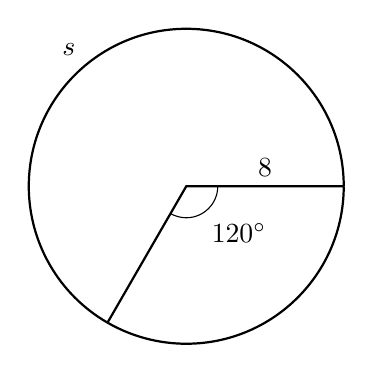
\begin{tikzpicture}[y=2cm, x=2cm,font=\sffamily]
  \draw[thick,black] (0:1) arc (0:240:1);
  \draw[thick,black] (0:1) -- (0,0) -- (240:1);
  \draw[thick,black] (0:1) arc (0:-120:1);

  \draw[black] (0.2,0) arc (0:-120:0.2);
  \node[anchor=south east] at (130:1) {$s$};
  \node[anchor=north west] at (300:0.2) {$120^\circ$};
  \node[anchor=south] at (0.5,0) {$8$};
\end{tikzpicture}


\end{enumerate}



\preClass{Coordinate Systems}


\videoLink{Section 4.5 day 1}{https://www.youtube.com/playlist?list=PLYHZK3b8UFw0U_iMosD8HZraus76s5k2i}

\begin{enumerate}
\item Let $f(x)=2\sin\left(3x-\frac{\pi}{2}\right)$.

\begin{enumerate}

\item  Determine the period, amplitude, and phase shift of $f(x)=2\sin\left(3x-\frac{\pi}{2}\right)$.\vfill
\item Find an interval containing exactly one cycle (period).\vfill
\item  Determine the $x$-values of the five key points in the cycle above.
$$x_1= \quad \quad \quad \quad x_2= \quad \quad \quad \quad x_3= \quad \quad \quad \quad x_4= \quad \quad \quad \quad x_5= \quad \quad \quad \quad$$
\vfill

\end{enumerate}
\clearpage


\item (2 points) Graph $f(x)=2\sin(3x-\frac{\pi}{2})$.

\begin{tikzpicture}[y=1cm, x=1.5cm,font=\sffamily]
    %% ticks
    \draw[step = 1, gray] (-5,-5) grid (5,5);
    %% axis
    \draw[thick,->] (-5.5,0) -- coordinate (x axis mid) (5.5,0) node[anchor = north west] {$x$};
    \draw[thick,->] (0,-5.5) -- coordinate (y axis mid) (0,5.5) node[anchor = north east] {$y$};
    \foreach \y in {-6,-5,...,-1,1,2,...,6} {
      \draw (2pt, \y) -- (-2pt, \y);
    }
    \foreach \x in {-6,-5,...,-1,1,2,...,6} {
      \draw (\x,2pt) -- (\x,-2pt);
    }

  \end{tikzpicture}







\item  Determine the period, amplitude, and phase shift of $f(x)=-7\cos(\pi x -4)$\vfill





\end{enumerate}






\actTitle{Worksheet 4.5A}

\noindent \textbf{Instructions:}  Work together in groups of  3 or 4 to complete the following problems.\\

Student goals:
\begin{itemize}
\item Determine the range and domain of a sine or a cosine function.
\item Determine the amplitude, period, and phase of a trigonometric
  function given a written or graphical representation.
\item Determine the vertical shift and scale of a trigonometric
  function given a written or graphical representation.
\item Graph a sine or cosine wave given a formula or written
  description.
\item Determine the formula for a sine or cosine wave given the
  graph or a written description of the function.
\end{itemize}

\begin{enumerate}

\item Determine the amplitude and period of the function.
\begin{enumerate}
\item $y=7\sin(2x)$ \vfill
\item $\displaystyle y=\frac{1}{7}\sin(2\pi x)$ \vfill
\item $\displaystyle y=-7\cos\left(-\frac{2}{3}x\right)$ \vfill
\end{enumerate}

\item Identify the phase shift and indicate whether the shift is to the left or to the right.
\begin{enumerate}
\item $\displaystyle \cos\left(x-\frac{\pi}{3}\right)$\vfill
\item $\displaystyle \cos\left(2x+\frac{\pi}{3}\right)$\vfill
\item $\displaystyle \sin\left(2\pi x -\frac{\pi}{8}\right)$\vfill
\end{enumerate}


\clearpage

\item Let $f(x)=2\cos(x+\pi)-1$.

\begin{enumerate}

\item Determine the period, amplitude, and phase shift of $f(x)=2\cos(x+\pi)-1$.\vfill
\item Find an interval containing exactly one cycle (period).\vfill
\item Determine the $x$-values of the five key points in the cycle above.
$$x_1= \quad \quad \quad \quad x_2= \quad \quad \quad \quad x_3= \quad \quad \quad \quad x_4= \quad \quad \quad \quad x_5= \quad \quad \quad \quad$$
\vfill





\item Graph $f(x)=2\cos(x+\pi)-1$.

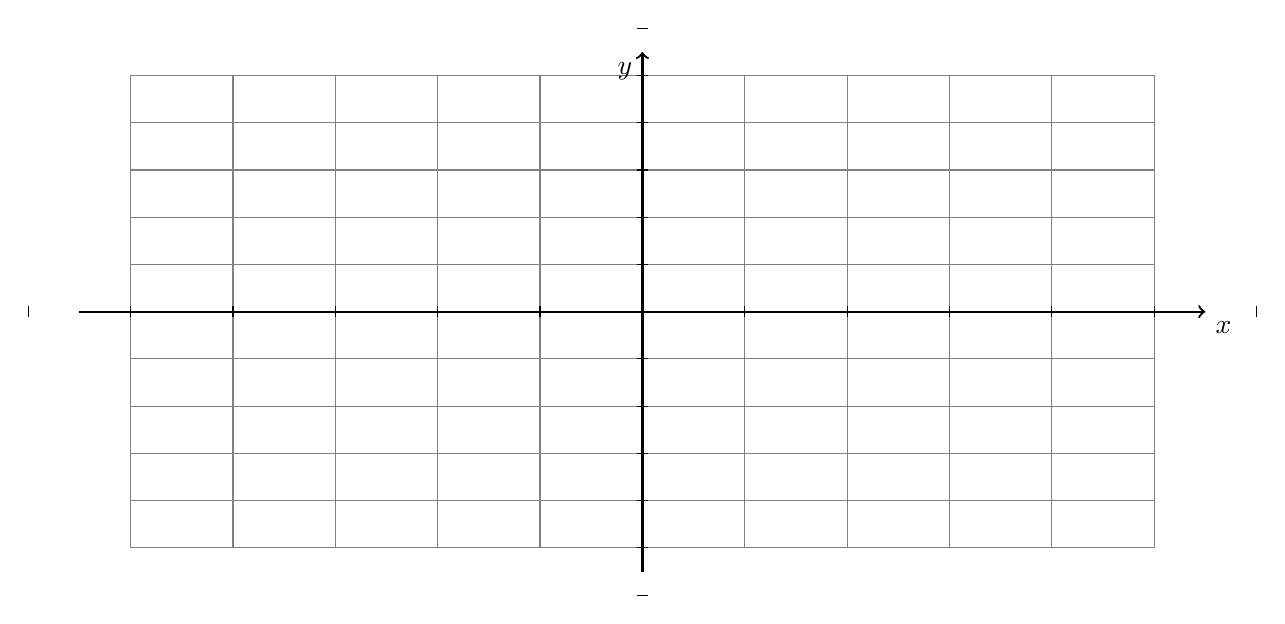
\begin{tikzpicture}[y=.6cm, x=1.3cm,font=\sffamily]
    %% ticks
    \draw[step = 1, gray] (-5,-5) grid (5,5);
    %% axis
    \draw[thick,->] (-5.5,0) -- coordinate (x axis mid) (5.5,0) node[anchor = north west] {$x$};
    \draw[thick,->] (0,-5.5) -- coordinate (y axis mid) (0,5.5) node[anchor = north east] {$y$};
    \foreach \y in {-6,-5,...,-1,1,2,...,6} {
      \draw (2pt, \y) -- (-2pt, \y);
    }
    \foreach \x in {-6,-5,...,-1,1,2,...,6} {
      \draw (\x,2pt) -- (\x,-2pt);
    }

  \end{tikzpicture}

\end{enumerate}


\clearpage

\item The function $y=a\sin(x)+d$ has range $[-10,28]$.  Assuming that $a$ is positive, determine the values for $a$ and $d$.

\vfill
\item The function $y=a\cos(x)+d$ has range $[-26,10]$.  Assuming that $a$ is positive, determine the values for $a$ and $d$.
\vfill

\item Let $f(x)=-7\sin(6x)$.
\begin{enumerate}
\item Determine the coordinates $(x,y)$ of the first maximum turning point on the graph $f(x)$ in the interval $(0,2\pi)$.
\vfill

\item Determine the coordinates $(x,y)$ of the first minimum turning point on the graph $f(x)$ in the interval $(0,2\pi)$.
\vfill

\end{enumerate}

\clearpage

\item The displacement of one of the vibrating wires in a piano is
  \begin{eqnarray*}
    D(t) & = & 0.05\cos\left(0.1\frac{\sqrt{T}}{L} t \right),
  \end{eqnarray*}
  where $T$ is the tension in the wire (measured in Newtons), $L$ is
  the length of the wire (meters), and $t$ is the time. A piano maker
  wishes to make a wire that vibrates 500 cycles per second, and the
  length of the wire will be 0.9 meters. What tension will be
  required?



\end{enumerate}


\hwTitle{Section 4.5A}

\begin{enumerate}
\item Let $\displaystyle f(x)=-5\sin\left(\frac{1}{3}x+\frac{\pi}{6}\right)$.

\begin{enumerate}

\item Determine the period, amplitude, and phase shift of
  $\displaystyle f(x)=-5\sin\left(\frac{1}{3}x+\frac{\pi}{6}\right)$.
\item Find an interval containing exactly one cycle (period).
\item Determine the $x$-values of the five key points in the cycle above.
$$x_1= \quad \quad \quad \quad x_2= \quad \quad \quad \quad x_3= \quad \quad \quad \quad x_4= \quad \quad \quad \quad x_5= \quad \quad \quad \quad$$
\item Graph $\displaystyle f(x)=-5\sin\left(\frac{1}{3}x+\frac{\pi}{6}\right)$.

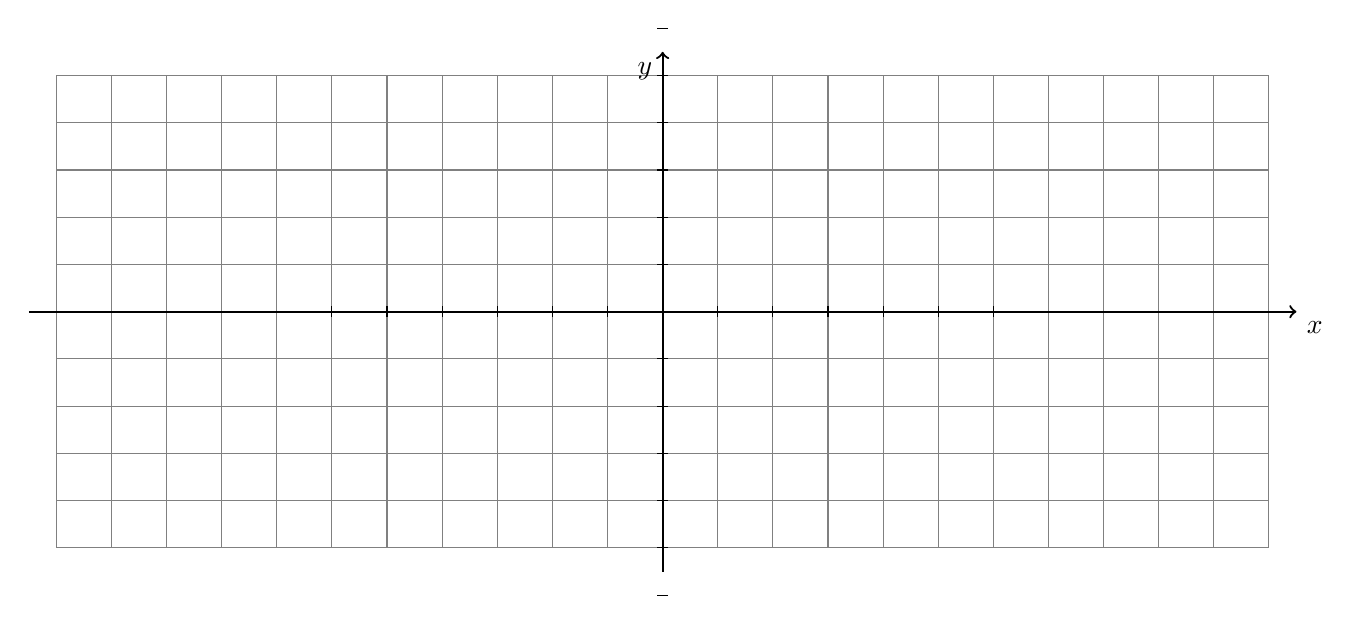
\begin{tikzpicture}[y=.6cm, x=.7cm,font=\sffamily]
    %% ticks
    \draw[step = 1, gray] (-11,-5) grid (11,5);
    %% axis
    \draw[thick,->] (-11.5,0) -- coordinate (x axis mid) (11.5,0) node[anchor = north west] {$x$};
    \draw[thick,->] (0,-5.5) -- coordinate (y axis mid) (0,5.5) node[anchor = north east] {$y$};
    \foreach \y in {-6,-5,...,-1,1,2,...,6} {
      \draw (2pt, \y) -- (-2pt, \y);
    }
    \foreach \x in {-6,-5,...,-1,1,2,...,6} {
      \draw (\x,2pt) -- (\x,-2pt);
    }

  \end{tikzpicture}

\end{enumerate}


\end{enumerate}


\preClass{Coordinate Systems}


\videoLink{Section 4.5 day 2}{https://www.youtube.com/playlist?list=PLYHZK3b8UFw0U_iMosD8HZraus76s5k2i}

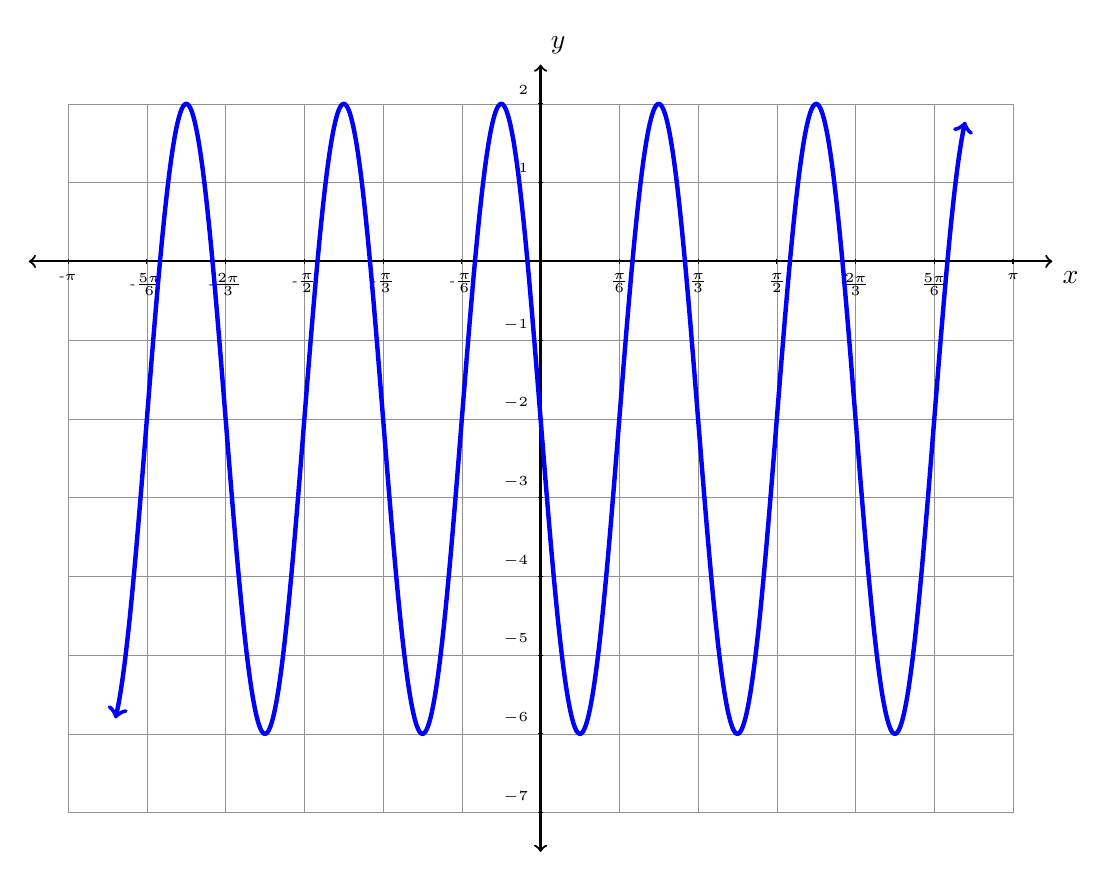
\begin{tikzpicture}[y=1cm, x=1cm,font=\sffamily,
	mydot/.style={
    circle,
    fill=white,
    draw,
    outer sep=0pt,
    inner sep=1.5pt
  }]
    %% Add a grid
    \draw[step = 1, gray, very thin,opacity=0.85] (-6, -7) grid (6, 2);
 	%% Draw the axes
	\draw[thick,<->] (-6.5,0) -- coordinate (x axis mid) (6.5,0) node[anchor = north west] {$x$};
    \draw[thick,<->] (0,-7.5) -- coordinate (y axis mid) (0,2.5) node[anchor = south west] {$y$};
    %% Label the y axis
    \foreach \y in {-7,...,-1,1,2,...,2} {
      \draw (1pt, \y) -- (-1pt, \y) node[anchor = south east] {\tiny $\y$};
    }
    %% Label the x axis
    %\foreach \x in {-5,...,-1,1,2,...,5} {
    %  \draw (\x,1pt) -- (\x,-1pt) node[anchor = north] {\tiny $\x$};
    %}
    \draw (-6,1pt) -- (-6,-1pt) node[anchor = north] {\tiny -$\pi$};
    \draw (-5,1pt) -- (-5,-1pt) node[anchor = north] {\tiny -$\frac{5\pi}{6}$};
    \draw (-4,1pt) -- (-4,-1pt) node[anchor = north] {\tiny -$\frac{2\pi}{3}$};
    \draw (-3,1pt) -- (-3,-1pt) node[anchor = north] {\tiny -$\frac{\pi}{2}$};
    \draw (-2,1pt) -- (-2,-1pt) node[anchor = north] {\tiny -$\frac{\pi}{3}$};
    \draw (-1,1pt) -- (-1,-1pt) node[anchor = north] {\tiny -$\frac{\pi}{6}$};
    \draw (1,1pt) -- (1,-1pt) node[anchor = north] {\tiny $\frac{\pi}{6}$};
    \draw (2,1pt) -- (2,-1pt) node[anchor = north] {\tiny $\frac{\pi}{3}$};
    \draw (3,1pt) -- (3,-1pt) node[anchor = north] {\tiny $\frac{\pi}{2}$};
    \draw (4,1pt) -- (4,-1pt) node[anchor = north] {\tiny $\frac{2\pi}{3}$};
    \draw (5,1pt) -- (5,-1pt) node[anchor = north] {\tiny $\frac{5\pi}{6}$};
    \draw (6,1pt) -- (6,-1pt) node[anchor = north] {\tiny $\pi$};

    %% Draw the function.
    \begin{scope}
%         \draw[very thick,blue] (-3,2) -- (1,1);
%         \draw[very thick,blue] (3.05,1.05) -- (4,3);
%         \draw[very thick,blue] (1.1,4) -- (3,4);
    %semi-circle
         %\draw[very thick, blue] (1,1) arc [radius=1, start angle=180, end angle= 5];
     %parabola
         %\draw[ultra thick, blue, domain=-5:0] plot (\x, {(-0.2)*(\x-5)*(\x+5)});
         \draw[ultra thick, blue, <->, domain=-5.4:5.4] plot[samples=1000] (\x, {-4*sin(pi*\x r)-2});             %dots
%         \fill[blue] (-3, 2) circle[radius=0.5ex];
%         \fill[blue] (1,1) circle[radius=0.5ex];
%         \fill[blue] (4,3) circle[radius=0.5ex];
%         \draw[very thick, blue] (3,1) circle[radius=0.5ex];
%         \fill[blue] (3,4) circle[radius=0.5ex];
%         \draw[very thick, blue] (1,4) circle[radius=0.5ex];


    \end{scope}

    %%\node[above=0.1cm] at (-2,2 )   {\nextXValue};

\end{tikzpicture}


\begin{enumerate}
\item  The graph above is a \textbf{sine} graph that has been transformed.   
\begin{enumerate}

\item  Determine the amplitude, period, phase shift, and vertical shift of function above.

{\bf Amplitude}: \hfill {\bf Period}:\hfill.

\vspace{1cm}

{\bf Phase Shift}: \hfill {\bf Vertical Shift}:\hfill.


\vspace{1cm}
\item  Determine a formula for $f(x)=A\sin(Bx+C)+D$ for the graph above. \vfill
	\vfill
 


\end{enumerate}



\end{enumerate}






\actTitle{Worksheet 4.5B}

\noindent \textbf{Instructions:}  Work together in groups of  3 or 4 to complete the following problems.\\

\begin{enumerate}

\item Write an equation of the form $A\cos(Bx+C)+D$ for the given graph where $A>0$ and  $B>0$.
\begin{center}
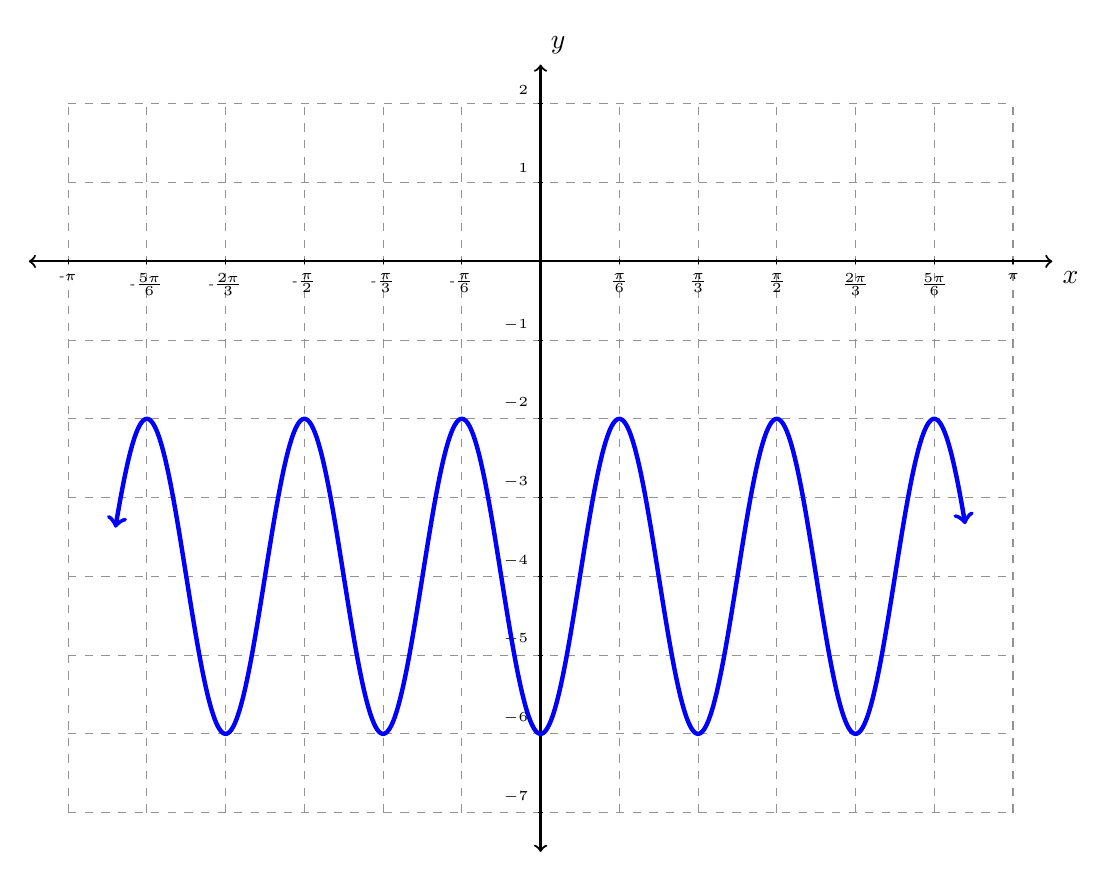
\begin{tikzpicture}[y=1cm, x=1cm,font=\sffamily,
	mydot/.style={
    circle,
    fill=white,
    draw,
    outer sep=0pt,
    inner sep=1.5pt
  }]
    %% Add a grid
    \draw[step = 1, gray, dashed,opacity=0.85] (-6, -7) grid (6, 2);
 	%% Draw the axes
	\draw[thick,<->] (-6.5,0) -- coordinate (x axis mid) (6.5,0) node[anchor = north west] {$x$};
    \draw[thick,<->] (0,-7.5) -- coordinate (y axis mid) (0,2.5) node[anchor = south west] {$y$};
    %% Label the y axis
    \foreach \y in {-7,...,-1,1,2,...,2} {
      \draw (1pt, \y) -- (-1pt, \y) node[anchor = south east] {\tiny $\y$};
    }
    %% Label the x axis
    %\foreach \x in {-5,...,-1,1,2,...,5} {
    %  \draw (\x,1pt) -- (\x,-1pt) node[anchor = north] {\tiny $\x$};
    %}
    \draw (-6,1pt) -- (-6,-1pt) node[anchor = north] {\tiny -$\pi$};
    \draw (-5,1pt) -- (-5,-1pt) node[anchor = north] {\tiny -$\frac{5\pi}{6}$};
    \draw (-4,1pt) -- (-4,-1pt) node[anchor = north] {\tiny -$\frac{2\pi}{3}$};
    \draw (-3,1pt) -- (-3,-1pt) node[anchor = north] {\tiny -$\frac{\pi}{2}$};
    \draw (-2,1pt) -- (-2,-1pt) node[anchor = north] {\tiny -$\frac{\pi}{3}$};
    \draw (-1,1pt) -- (-1,-1pt) node[anchor = north] {\tiny -$\frac{\pi}{6}$};
    \draw (1,1pt) -- (1,-1pt) node[anchor = north] {\tiny $\frac{\pi}{6}$};
    \draw (2,1pt) -- (2,-1pt) node[anchor = north] {\tiny $\frac{\pi}{3}$};
    \draw (3,1pt) -- (3,-1pt) node[anchor = north] {\tiny $\frac{\pi}{2}$};
    \draw (4,1pt) -- (4,-1pt) node[anchor = north] {\tiny $\frac{2\pi}{3}$};
    \draw (5,1pt) -- (5,-1pt) node[anchor = north] {\tiny $\frac{5\pi}{6}$};
    \draw (6,1pt) -- (6,-1pt) node[anchor = north] {\tiny $\pi$};

    %% Draw the function.
    \begin{scope}
%         \draw[very thick,blue] (-3,2) -- (1,1);
%         \draw[very thick,blue] (3.05,1.05) -- (4,3);
%         \draw[very thick,blue] (1.1,4) -- (3,4);
    %semi-circle
         %\draw[very thick, blue] (1,1) arc [radius=1, start angle=180, end angle= 5];
     %parabola
         %\draw[ultra thick, blue, domain=-5:0] plot (\x, {(-0.2)*(\x-5)*(\x+5)});
         \draw[ultra thick, blue, <->, domain=-5.4:5.4] plot[samples=1000] (\x, {-2*cos(pi*\x r)-4});             %dots
%         \fill[blue] (-3, 2) circle[radius=0.5ex];
%         \fill[blue] (1,1) circle[radius=0.5ex];
%         \fill[blue] (4,3) circle[radius=0.5ex];
%         \draw[very thick, blue] (3,1) circle[radius=0.5ex];
%         \fill[blue] (3,4) circle[radius=0.5ex];
%         \draw[very thick, blue] (1,4) circle[radius=0.5ex];


    \end{scope}

    %%\node[above=0.1cm] at (-2,2 )   {\nextXValue};

\end{tikzpicture}

\end{center}

\vfill


\clearpage
\item Write an equation of the form $A\sin(Bx+C)+D$ for the given graph where $A>0$ and  $B>0$.
\begin{center}
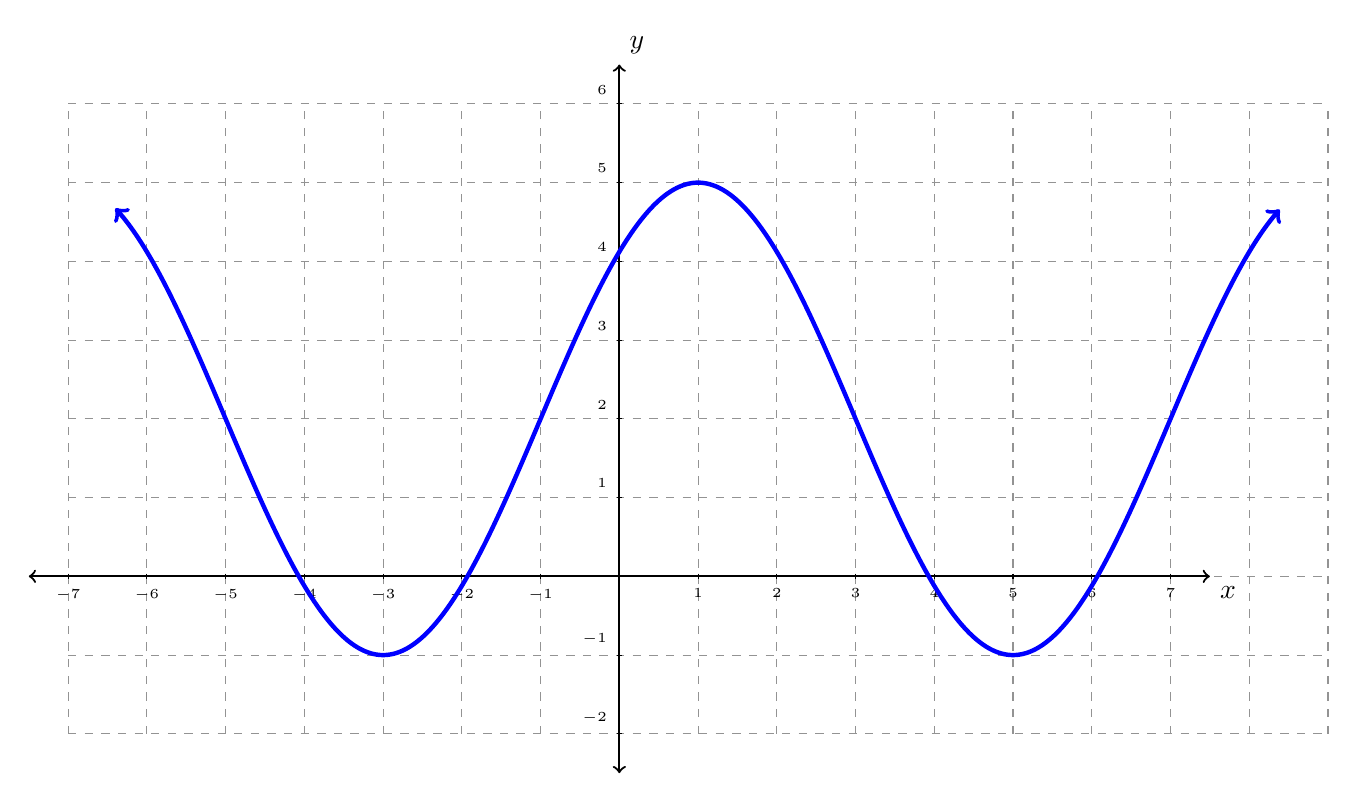
\begin{tikzpicture}[y=1cm, x=1cm,font=\sffamily,
	mydot/.style={
    circle,
    fill=white,
    draw,
    outer sep=0pt,
    inner sep=1.5pt
  }]
    %% Add a grid
    \draw[step = 1, gray,dashed,opacity=0.85] (-7, -2) grid (9, 6);
 	%% Draw the axes
	\draw[thick,<->] (-7.5,0) -- coordinate (x axis mid) (7.5,0) node[anchor = north west] {$x$};
    \draw[thick,<->] (0,-2.5) -- coordinate (y axis mid) (0,6.5) node[anchor = south west] {$y$};
    %% Label the y axis
    \foreach \y in {-2,...,-1,1,2,...,5,6} {
      \draw (1pt, \y) -- (-1pt, \y) node[anchor = south east] {\tiny $\y$};
    }
    %% Label the x axis
    \foreach \x in {-7,...,-1,1,2,...,7} {
      \draw (\x,1pt) -- (\x,-1pt) node[anchor = north] {\tiny $\x$};
    }
    %% Draw the function.
    \begin{scope}
%         \draw[very thick,blue] (-3,2) -- (1,1);
%         \draw[very thick,blue] (3.05,1.05) -- (4,3);
%         \draw[very thick,blue] (1.1,4) -- (3,4);
    %semi-circle
         %\draw[very thick, blue] (1,1) arc [radius=1, start angle=180, end angle= 5];
     %parabola
         %\draw[ultra thick, blue, domain=-5:0] plot (\x, {(-0.2)*(\x-5)*(\x+5)});
         \draw[ultra thick, blue, <->, domain=-6.4:8.4] plot[samples=1000] (\x, {3*sin(pi/4*(\x+1) r)+2});             %dots
%         \fill[blue] (-3, 2) circle[radius=0.5ex];
%         \fill[blue] (1,1) circle[radius=0.5ex];
%         \fill[blue] (4,3) circle[radius=0.5ex];
%         \draw[very thick, blue] (3,1) circle[radius=0.5ex];
%         \fill[blue] (3,4) circle[radius=0.5ex];
%         \draw[very thick, blue] (1,4) circle[radius=0.5ex];


    \end{scope}

    %%\node[above=0.1cm] at (-2,2 )   {\nextXValue};

\end{tikzpicture}

\end{center}


\vfill

\clearpage
\item Write equations of the form $A\sin(Bx+C)+D$ \textbf{AND} $A\cos(Bx+C)+D$ and for the given graph where $A>0$ and  $B>0$.
\begin{center}
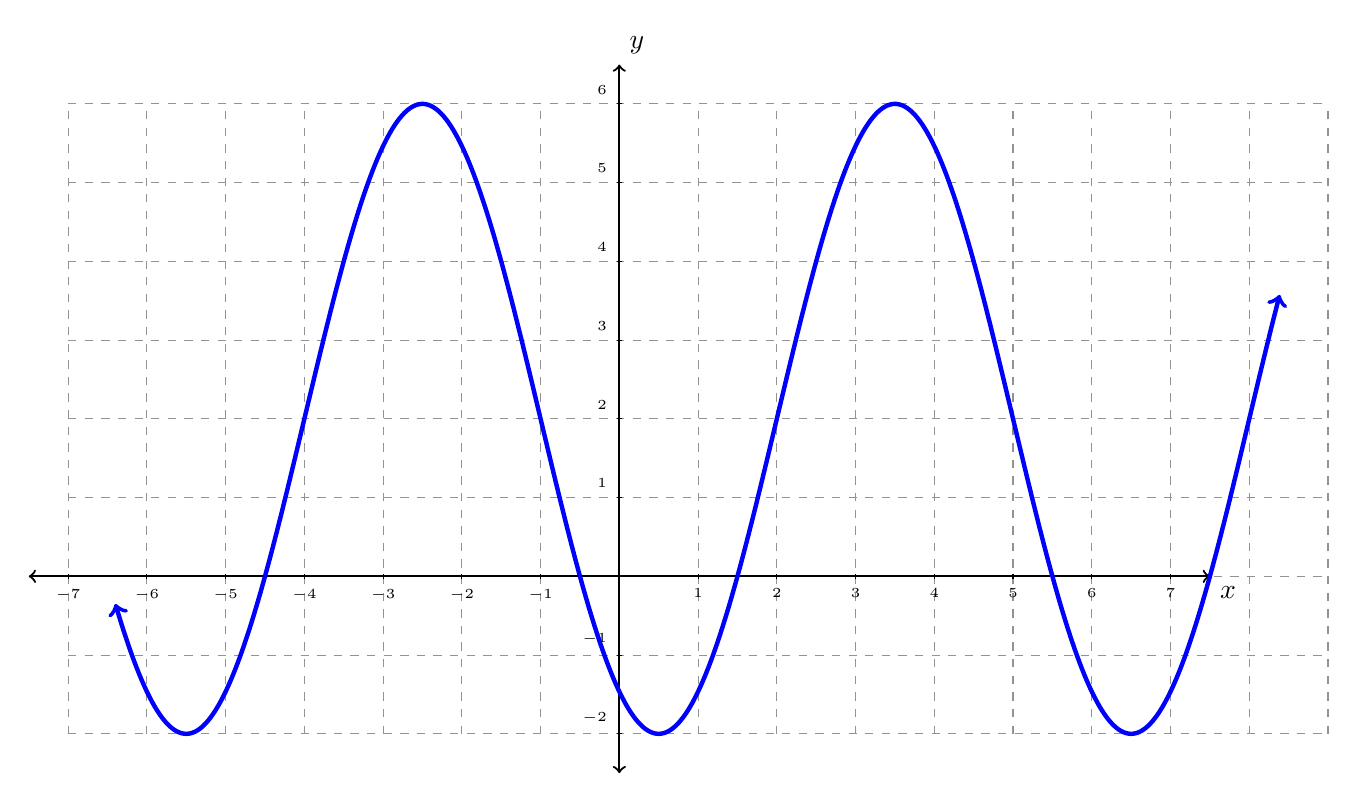
\begin{tikzpicture}[y=1cm, x=1cm,font=\sffamily,
	mydot/.style={
    circle,
    fill=white,
    draw,
    outer sep=0pt,
    inner sep=1.5pt
  }]
    %% Add a grid
    \draw[step = 1, gray,dashed,opacity=0.85] (-7, -2) grid (9, 6);
 	%% Draw the axes
	\draw[thick,<->] (-7.5,0) -- coordinate (x axis mid) (7.5,0) node[anchor = north west] {$x$};
    \draw[thick,<->] (0,-2.5) -- coordinate (y axis mid) (0,6.5) node[anchor = south west] {$y$};
    %% Label the y axis
    \foreach \y in {-2,...,-1,1,2,...,5,6} {
      \draw (1pt, \y) -- (-1pt, \y) node[anchor = south east] {\tiny $\y$};
    }
    %% Label the x axis
    \foreach \x in {-7,...,-1,1,2,...,7} {
      \draw (\x,1pt) -- (\x,-1pt) node[anchor = north] {\tiny $\x$};
    }
    %% Draw the function.
    \begin{scope}
%         \draw[very thick,blue] (-3,2) -- (1,1);
%         \draw[very thick,blue] (3.05,1.05) -- (4,3);
%         \draw[very thick,blue] (1.1,4) -- (3,4);
    %semi-circle
         %\draw[very thick, blue] (1,1) arc [radius=1, start angle=180, end angle= 5];
     %parabola
         %\draw[ultra thick, blue, domain=-5:0] plot (\x, {(-0.2)*(\x-5)*(\x+5)});
          \draw[ultra thick, blue, <->, domain=-6.4:8.4] plot[samples=1000] (\x, {-4*sin(pi/3*(\x+1) r)+2});             %dots
%         \fill[blue] (-3, 2) circle[radius=0.5ex];
%         \fill[blue] (1,1) circle[radius=0.5ex];
%         \fill[blue] (4,3) circle[radius=0.5ex];
%         \draw[very thick, blue] (3,1) circle[radius=0.5ex];
%         \fill[blue] (3,4) circle[radius=0.5ex];
%         \draw[very thick, blue] (1,4) circle[radius=0.5ex];


    \end{scope}

    %%\node[above=0.1cm] at (-2,2 )   {\nextXValue};

\end{tikzpicture}

\end{center}


\vfill




\clearpage
\item The water level relative to the top of a boat dock varies with
  the tides.  One particular day, low tide occurs at midnight and the
  water level is 7ft below the dock.  The first high tide of the day
  occurs at approximately 6:00 AM, and the water level is 3ft below
  the dock.  The next low tide occurs at noon and the water level is
  again 7ft below the dock.
  
  Assuming that this pattern continues indefinitely and behaves like a
  cosine wave, write a function of the form $w(t)=A\cos(Bt+C)+D$.  The
  value $w(t)$ is the water level (in ft) relative to the top of the
  dock, $t$ hours after midnight.

  \vfill

\clearpage

\item The function $f(x)=A\sin(Bx)+D$ has a period of $13\pi$.  If the graph of $f(x)$ oscillates between 2 and 20, determine the numeric values for A, B, and D.  (You may assume that A, B, and D are positive.)
\vfill
\vfill

\item Write the range of the function in interval notation.
\begin{enumerate}
\item $y=\sin(x)$\\[0.2in]
\item $y=\cos(x)$\\[0.2in]
\item $y=8\cos(2x-\pi)+4$\vfill
\end{enumerate}

\clearpage


\item The London Eye is a Ferris wheel with a diameter of 120
  meters. The center of the wheel is 75 meters above the ground, and
  the wheel makes one revolution every thirty minutes. If one of the
  capsules is initially at the lowest level at the initial time,
  determine a function that returns the height of the capsule above
  the ground given the number of minutes after the initial time.

  \vfill


\end{enumerate}


\hwTitle{Section 4.5B}

\begin{enumerate}
\item Write the range of the function in interval notation.
\begin{enumerate}
\item $y=-3\cos\left(x+\frac{\pi}{3}\right)-5$
\item $y=-6\sin\left(3x-\frac{\pi}{2}\right)-2$
\item $y=-\sin(x)$
\item $y=-5\cos(2x+1)+ 10$
\item $y=20\cos\left(5x-\frac{\pi}{5}\right)+20$
\end{enumerate}

\item Graph $f(x)=-6\sin\left(3x-\frac{\pi}{2}\right)-2$.

\begin{tikzpicture}[y=.6cm, x=1.3cm,font=\sffamily]
    %% ticks
    \draw[step = 1, gray,dashed] (-5,-10) grid (5,10);
    %% axis
    \draw[thick,->] (-5.5,0) -- coordinate (x axis mid) (5.5,0) node[anchor = north west] {$x$};
    \draw[thick,->] (0,-10.5) -- coordinate (y axis mid) (0,10.5) node[anchor = north east] {$y$};
    %\foreach \y in {-10,-9,...,-1,1,2,...,10} {
    %  \draw (2pt, \y) -- (-2pt, \y);
    %}
    %\foreach \x in {-6,-5,...,-1,1,2,...,6} {
    %  \draw (\x,2pt) -- (\x,-2pt);
    %}

  \end{tikzpicture}

\item Determine a formula for the sine wave that oscillates between
  two and eight. It has a minimum at $x = 2$, and the wave repeats
  every five units (i.e. the period is five).

\item Determine a formula for the cosine wave that oscillates between
  minus five and twenty. It has a maximum at $x=6$, and the wave repeats
  every four units (i.e. the period is four).

\item The water level at a beach oscillates between 0.4m
  \textbf{below} the mean tidal level and 3.4m \textbf{above} the mean
  tidal level. The time between low and high tides is 6.4 hours. If
  low tide occurs at midnight, express the water level as a cosine
  function where the time is the number of hours past midnight,
  \begin{eqnarray*}
    h(t) & = & A \cos(bt+c)+d.
  \end{eqnarray*}

\item The water level at Jeffries Creek varies between 2.4 meters and
  0.2 meters due to the changes in the tide. The time between high
  tides is 700 minutes. The next high tide will occur at 150 minutes
  after midnight. Express the water level as a sine function assuming
  that $t=0$ minutes is midnight.

\item Determine the cosine function whose graph is shown below.

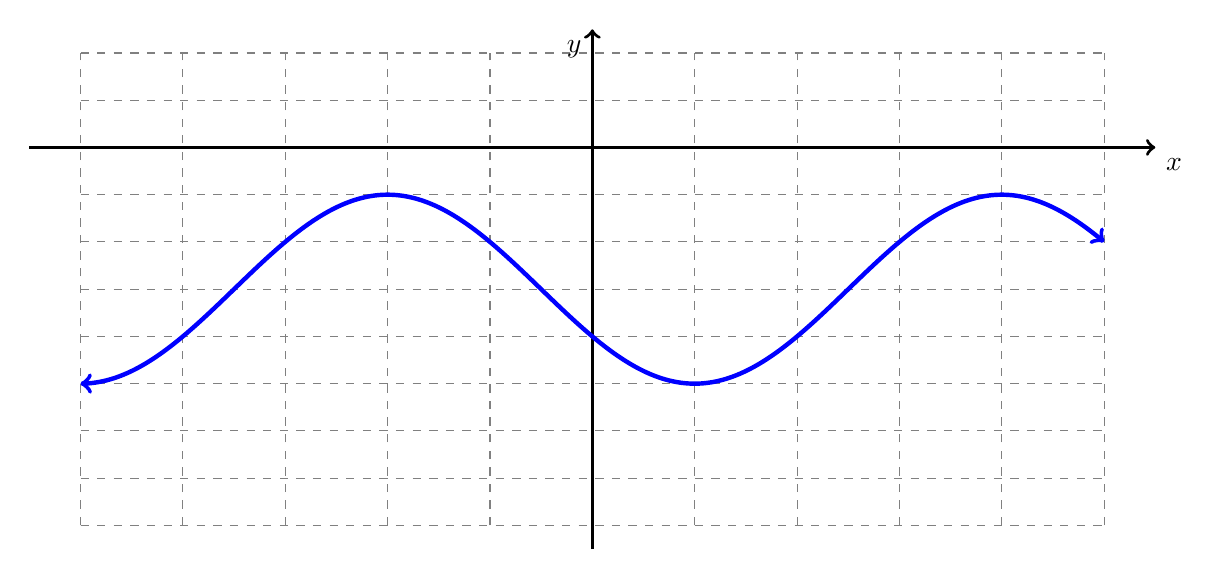
\begin{tikzpicture}[y=.6cm, x=1.3cm,font=\sffamily]
  %% ticks
  \draw[step = 1, gray,dashed] (-5,-8) grid (5,2);
  %% axis
  \draw[very thick,->] (-5.5,0) -- coordinate (x axis mid) (5.5,0) node[anchor = north west] {$x$};
  \draw[very thick,->] (0,-8.5) -- coordinate (y axis mid) (0,2.5) node[anchor = north east] {$y$};
  \draw[ultra thick, blue, <->, domain=-5:5] plot[samples=1000] (\x, {2*cos(deg(pi/3*(\x+2)))-3});
\end{tikzpicture}

\item The wheel used in the game show Wheel Of Fortune is
  approximately 2.6 meters in diameter. Suppose the Wheel is mounted
  vertically on a wall for a special event so that its center is 4
  meters above the floor. Initially, the 100\$ marker is to the right,
  and the Wheel is spun clock-wise so that it takes four seconds to
  make one revolution. Determine the height above the floor of the
  outside edge of the 100\$ marker given the number of seconds after
  the initial time.

\item The clock face of the Rajabai Tower is approximately 65 meters
  above the ground, and the length of the minute hand is approximately
  7.3 meters. A bird lands on the end of the minute hand at 3:45PM and
  remains on the minute for thirty minutes. Determine the bird's
  height above the ground given the number of minutes after 3:45PM.

\item The height above the ground (in meters) for the seats on a Ferris wheel is
  given by
  \begin{eqnarray*}
    H(t) & = & 27 \cos\left(\frac{\pi}{3}t+\pi\right) + 32,
  \end{eqnarray*}
  where $t$ is the time in minutes from the start of the
  ride. Determine how long it takes for one revolution to occur. How
  tall is the loading platform which is located at the bottom of the
  wheel? What is the maximum height of one of the seats?


\end{enumerate}


\preClass{Coordinate Systems}


\videoLink{Section 4.7 day 1}{https://www.youtube.com/playlist?list=PLYHZK3b8UFw084fqUEZ7lpLyl4MJiCOwu}

\begin{enumerate}
\item  Find the exact value of the following inverse functions.

\begin{enumerate}
\item $\displaystyle \cos^{-1}\Big(\frac{\sqrt{2}}{2}\Big)$\vfill
\item $\displaystyle \sin^{-1}\Big(-\frac{\sqrt{2}}{2}\Big)$\vfill
\item $\displaystyle \tan^{-1}(-1)$\vfill

\end{enumerate}
\newpage


\item  Find the exact value of the expression.  Do not use a calculator.

\begin{enumerate}
\item $\sin(\sin^{-1}(1))$\vfill
\item $\displaystyle \sin^{-1}\Big(\sin\Big(\frac{7\pi}{6}\Big)\Big)$\vfill
\end{enumerate}

\item  Find the exact value of the expression.  Do not use a calculator.

\begin{enumerate}
\item $\cos(\cos^{-1}(1))$\vfill
\item $\displaystyle \cos^{-1}(\cos(1))$\vfill
\end{enumerate}
\end{enumerate}






\actTitle{Worksheet 4.7A}

\noindent \textbf{Instructions:}  Work together in groups of  3 or 4
to complete the following problems.

Student goals:
\begin{itemize}
\item Determine the restriction of the domain of a function in order
  to define an inverse.
\item State the canonical domain restrictions for sine, cosine, and
  tangent functions.
\item Use the definition of the arcsine, arccosine, and the arctangent
  functions to solve for one value in a trigonometric expression.
\item Sketch the graphs of the arcsine, arccosine, and the arctangent
  functions.
\item Compose trigonometric and inverse trigonometric functions to
  transform a trigonometric expression into an equivalent form that
  allows for direct algebraic manipulation to isolate a value in the
  domain of a trigonometric function in the original expression.
\item Determine equivalent expressions for the compositions of
  trigonometric and inverse trigonometric functions so that the
  results do not include any trigonometric functions.
\end{itemize}


\begin{enumerate}

\item Use the unit circle/reference triangles to determine the value of each of the following.
\begin{enumerate}
\item $\arcsin \left( \frac{\sqrt{2}}{2}\right)$
  \vfill
\item $\sin^{-1} \left( -\frac{\sqrt{3}}{2}\right)$
  \vfill
\item $\sin^{-1} \left( \frac{\sqrt{3}}{2}\right)$
  \vfill
\item $\arcsin \left( -\frac{1}{2}\right)$
  \vfill
\end{enumerate}


\item Use the unit circle/reference triangles to determine the value of each of the following.
\begin{enumerate}
\item $\arccos \left( \frac{\sqrt{2}}{2}\right)$
  \vfill
\item $\cos^{-1} \left( -\frac{\sqrt{3}}{2}\right)$
  \vfill
\item $\cos^{-1} \left( \frac{\sqrt{3}}{2}\right)$
  \vfill
\item $\arccos \left( -\frac{1}{2}\right)$
  \vfill
\end{enumerate}

\clearpage

\item Use the unit circle/reference triangles to determine the value of each of the following.
\begin{enumerate}
\item $\arctan \left( 1 \right)$
  \vfill
\item $\tan^{-1} \left( \frac{1}{\sqrt{3}}\right)$
  \vfill
\item $\tan^{-1} \left(\sqrt{3}\right)$
  \vfill
\item $\arctan \left( -1 \right)$
  \vfill
\end{enumerate}


\item Find the exact value of the expression.  Do not use a calculator.

\begin{enumerate}

\item $\arcsin \left(\sin\left(\frac{\pi}{3}\right)\right)=$
\vfill

\item $\arcsin \left(\sin\left(\frac{5\pi}{4}\right)\right)=$
\vfill

\item $\arccos \left(\cos\left(\frac{11\pi}{6}\right)\right)=$
\vfill


\item $\cos \left(\arccos\left( 0.56 \right)\right) = $
\vfill

\item $\tan \left( \arctan\left(1754\right) \right)=$
\vfill

\item $\arctan \left( \tan\left( \frac{23}{814}\right)\right)=$
\vfill

\end{enumerate}


\clearpage

\item Use a calculator to approximate the degree measure (to 1 decimal place) or radian measure (to 4 decimal places) of the angle $\theta$ subject to the given conditions. (\textbf{Hint:  }Use reference angles!)

\begin{enumerate}
\item $\displaystyle \cos(\theta)=-\frac{8}{11}$ and $180^\circ \leq \theta \leq 270^\circ$
\vfill
\item $\displaystyle \tan(\theta)=-\frac{9}{7}$ and $\frac{\pi}{2}<\theta< \pi$
\vfill
\item $\displaystyle \sin(\theta)=\frac{12}{19}$ and $90^\circ < \theta <180^\circ$
\vfill
\end{enumerate}


\clearpage



\item A student measures the length of the shadow of the Washington
  Monument to be 620 ft. If the Washington Monument is 555 ft tall,
  approximate the angle of elevation of the Sun to the nearest tenth
  of a degree.

  \vfill

\item A balloon advertising an open house is stabilized by two cables
  of lengths 20 ft and 40 ft tethered to the ground.  If the
  perpendicular distance from the balloon to the ground is
  $10\sqrt{3}$ ft, what is the degree measure of the angle each cable
  makes with the ground?  Round to the nearest tenth of a
  \textbf{degree} if necessary.

  \vfill


\end{enumerate}


\preClass{Coordinate Systems}


\videoLink{Section 4.7 day 2}{https://www.youtube.com/playlist?list=PLYHZK3b8UFw0JZy4oRGwxyv_LaTgWK5r2}


\begin{enumerate}


\item  Determine the exact value of the following.  Show all work.
  $$\sin\left(\tan^{-1}\left(\frac{12}{5}\right)\right)$$
  \vfill
\item Determine the exact value of the following.  Show all work.
  $$\cos\left(\sin^{-1}\left(-\frac{2}{11}\right)\right)$$
  \vfill
\end{enumerate}






\actTitle{Worksheet 4.7B}

\noindent \textbf{Instructions:}  Work together in groups of  3 or 4 to complete the following problems.\\

\begin{enumerate}

\item Find the exact values of the following.
\begin{enumerate}

\item $\cos \left( \tan^{-1}(\frac{\sqrt{3}}{3})\right)$

\vfill
\item $\tan \left( \sin^{-1}(-\frac{2}{3})\right)$


\vfill

\item $\sin \left( \cos^{-1}(\frac{3}{4})\right)$
\vfill

\item $\sec \left( \tan^{-1}(\frac{4}{3})\right)$
\vfill

\end{enumerate}



\newpage
\item Write the expression as an \textbf{algebraic} expression.  (There should be no trig functions in your answers.)

\begin{enumerate}

\item $\displaystyle \sin \left( \cos^{-1}\left(\frac{\sqrt{x^2-25}}{x}\right)\right)$ for $x>5$

\vfill

\item $\displaystyle \tan \left( \cos^{-1}\left(\frac{3}{x}\right)\right)$ for $x>3$
\vfill

\item $\displaystyle \sin \left( \tan^{-1}\left(x\right)\right)$ for $x>0$
\vfill


\end{enumerate}


\newpage

\item A group of campers hike down a steep path.  One member of the group has an altimeter on his watch to measure altitude.  If the path is 1250 yd and the amount of altitude lost is 480 yd, what is the angle of incline?  Round to the nearest tenth of a \textbf{degree}.
\vfill

\item A video camera located at ground level follows the liftoff of an Atlas V Rocket from the Kennedy Space Center.  Suppose that the camera is 1000 m from the launch pad.
\begin{enumerate}
\item Write the angle of elevation $\theta$ from the camera to the rocket as a function of the rocket's height, $h$.
\vfill
\item Use a calculator to find $\theta$ to the nearest tenth of a degree when the rocket's height is 400 m, 1500 m, and 3000 m.
\vfill
\end{enumerate}

\newpage
\item Determine the value of $\theta$ associated with the coordinate
      in the figure below. (Numerical answers should be to within 2
      decimal digits.)

      \begin{tikzpicture}[y=1.0cm, x=1.0cm,font=\sffamily]
        \draw[thick,black] (-2,0) -- (2,0) node[anchor=west] {$x$};
        \draw[thick,black] (0,-2) -- (0,2) node[anchor=south] {$y$};
        \draw[thin,black] (0,0) -- (-1,-1.8);
        \draw[thin,black] (-0.3,0) arc (180:240:0.3);
        \node[black,xshift=-15.4,yshift=-8.2] at (0,0) {$\theta$};
        \node[black,anchor=north east] at (-1,-1.8) {$(-4,-4\sqrt{3})$};
        \draw[black,fill=black] (-1,-1.8) circle (0.5ex);
      \end{tikzpicture}

\item Determine the \textbf{exact} values of each of the
  expressions below. (Do not use a value from a calculator but derive the true value.)
  \begin{enumerate}


  \item
    ${\displaystyle \cos\left(\frac{\pi}{2} + \arcsin\left(\frac{3}{5}\right) \right) }$ 
    \vfill
    
   \item
    ${\displaystyle \cos\left(\pi + \arcsin\left(\frac{3}{5}\right) \right) }$ 
    \vfill
    
      \item
    ${\displaystyle \cos\left(2\pi - \arcsin\left(\frac{3}{5}\right) \right) }$ 
    \vfill   
    


  \end{enumerate}

\end{enumerate}



\preClass{Coordinate Systems}


\videoLink{Section 5.1}{https://www.youtube.com/playlist?list=PLYHZK3b8UFw0Afc951bZjITtow-fxztxp}

\begin{enumerate}
\item  Simplify the expression.  Write the final form with no fractions or products.
$$\cos(x)\tan(x)\csc(x)$$

\vfill

\item Verify the trigonometric identities and \textbf{write the name of the fundamental identity used at each step}. Remember to only manipulate one side.  The other side should stay the same.

\begin{enumerate}
\item  $\sin(-x)+\csc(x)=\cot(x)\cos(x)$\vfill
\vfill
\vfill


\clearpage

\item  $\displaystyle \frac{\sin^2(x)+1}{\cos^2(x)}+1=2\sec^2(x)$\vfill
\end{enumerate}

\end{enumerate}





\actTitle{Worksheet 5.1}

\noindent \textbf{Instructions:}  Work together in groups of  3 or 4 to complete the following problems.\\

\begin{enumerate}



\item Verify each identity.
\begin{enumerate}

\item $\cot(-x)\sin(-x)=\cos(x)$

\vfill
\item $\displaystyle \frac{\csc(x)-\sec(x)}{\csc(x)+\sec(x)}=\frac{\cot(x)-1}{\cot(x)+1}$

\vfill
\vfill
\newpage
\item $\displaystyle \frac{\tan(x)+\tan(y)}{\tan(x)\tan(y)-1}=\frac{\sin(x)\cos(y)+\cos(x)\sin(y)}{\sin(x)\sin(y)-\cos(x)\cos(y)}$
\vfill

\vfill

\end{enumerate}



\newpage
\item $$\tan(-x)\cos(x)=-\sin(x)$$
Choose the sequence of steps below that verifies the identity.

\begin{enumerate}

\item $\displaystyle \tan(-x)\cos(x)=-\tan(x)\cdot \cos(x)=-\frac{\cos(x)}{\sin(x)}\cdot \cos(x)=-\sin(x)$
\item $\displaystyle \tan(-x)\cos(x)=-\tan(x)\cdot \cos(x)=-\frac{\sin(x)}{\cos(x)}\cdot \cos(x)=-\sin(x)$
\item $\displaystyle \tan(-x)\cos(x)=\tan(x)\cdot -\cos(x)=\frac{\cos(x)}{\sin(x)}\cdot -\cos(x)=-\sin(x)$
\item $\displaystyle \tan(-x)\cos(x)=-\tan(x)\cdot -\cos(x)=-\frac{\sin(x)}{\cos(x)}\cdot -\cos(x)=-\sin(x)$

\vfill


\end{enumerate}

\item Choose the correct expression that completes the identity.
$$\frac{\cos^2(x)-\sin^2(x)}{1-\tan^2(x)}=$$
\begin{enumerate}
\item -1
\item 1
\item $\cos^2(x)$
\item $\sin^2(x)$
\end{enumerate}
\vfill
\newpage

\item Choose the correct expression that completes the identity.
$$\sin^4(x)-\cos^4(x)=$$
\begin{enumerate}
\item $1-2\cos^2(x)$
\item $1+2\cos^2(x)$
\item $1-2\sin^2(x)$
\item $1+2\sin^2(x)$
\end{enumerate}
\vfill

\item Verify the identity.

\begin{enumerate}
\item $\left(6\cos(\theta)-\sin(\theta)\right)^2+\left(\cos(\theta)+6\sin(\theta)\right)^2=37$.
\vfill
\item $\displaystyle \frac{(\sin(x)+\cos(x))^2}{1+2\sin(x)\cos(x)}=1$
\vfill
\end{enumerate}

\newpage


\item Rewrite the expression in terms of the given function.
\begin{enumerate}
\item $\displaystyle \frac{\tan(x)+\cot(x)}{\sec(x)}$ in terms of $\csc(x)$
\vfill
\item $\displaystyle \frac{\tan(x)}{-1+\sec(x)}-\frac{\sec(x)}{\tan(x)}$ in terms of $\tan(x)$
\vfill

\end{enumerate}

\newpage
\item Verify the identity.

\begin{enumerate}
\item $\tan^4(t)-\sec^4(t)=-2\tan^2(t)-1$
\vfill
\item $\displaystyle \csc(x)+\tan^2(x)\csc(x)=\frac{1}{\sin(x)\cos^2(x)}$
\vfill
\end{enumerate}






\end{enumerate}


\preClass{Coordinate Systems}


\videoLink{Section 5.2}{https://www.youtube.com/playlist?list=PLYHZK3b8UFw3NgZa9wBc8k8LS5w45veeB}

\begin{enumerate}
\item  Evaluate the following using a sum or difference identity and the unit circle.
$$\cos(165^\circ)$$

\vfill

\item  Find the exact value of $\cos (\alpha - \beta)$ given that $\sin \alpha = -\frac{4}{5}$ and $\cos \beta = -\frac{5}{8}$ for $\alpha$ in Quadrant III and $\beta$ in Quadrant II.
\vfill
\vfill


\newpage
\item  Find the exact value of the following.  $$\cos \left( \arcsin \left(-\frac{12}{37}\right)+\arctan \left(\frac{5}{12}\right)\right)$$
\vfill

\end{enumerate}






\actTitle{Worksheet 5.2}
\noindent \textbf{Instructions:}  Work together in groups of  3 or 4
to complete the following problems.

Student goals:
\begin{itemize}
\item Use the sum and difference formulas for the sine function to
  solve for values within a trigonometric expression.
\item Use the sum and difference formulas for the cosine function to
  solve for values within a trigonometric expression.
\item Verify identities that make use of sum and difference formulas.
\item Combine the sum and difference formulas with inverse
  trigonometric functions.
\end{itemize}



\begin{enumerate}



\item Write each expression as the sine, cosine, or tangent of an angle.  Then find the value the expression.
\begin{enumerate}
\item $\sin(10^\circ)\cos(80^\circ)+\cos(10^\circ)\sin(80^\circ)$
\vfill
\item $\displaystyle\sin\left(\frac{2\pi}{3}\right)\cos\left(\frac{\pi}{6}\right)-\cos\left(\frac{2\pi}{3}\right)\sin\left(\frac{\pi}{6}\right)$
\vfill
\item $\cos(71^\circ)\cos(19^\circ)-\sin(71^\circ)\sin(19^\circ)$
\vfill
\item $\displaystyle\cos\left(\frac{5\pi}{12}\right)\cos\left(\frac{\pi}{12}\right)+\sin\left(\frac{5\pi}{12}\right)\sin\left(\frac{\pi}{12}\right)$
\vfill
\newpage
\item $\displaystyle \frac{\tan(25^\circ)+\tan(20^\circ)}{1-\tan(25^\circ)\tan(20^\circ)}$
\vfill
\item $\displaystyle \frac{\tan\left(\frac{4\pi}{5}\right)-\tan\left(\frac{11\pi}{20}\right)}{1+\tan\left(\frac{4\pi}{5}\right)\tan\left(\frac{11\pi}{20}\right)}$
\vfill
\end{enumerate}


\item Find the exact value of each expression.

\begin{enumerate}

\item $\sin(105^\circ)$
\vfill
\item $\sin(15^\circ)$
\vfill

\newpage

\item $\displaystyle\cos\left(\frac{7\pi}{12}\right)$

\vfill
\item $\displaystyle \sin\left(\frac{\pi}{12}\right)$

\vfill


\item $\displaystyle \tan\left(\frac{\pi}{12}\right)$
\vfill


\end{enumerate}

\newpage

\item Find the exact value of $\sin(\alpha+\beta)$, $\cos(\alpha+\beta)$, and $\tan(\alpha+\beta)$ under the given conditions.

\begin{enumerate}
\item $\sin(\alpha)=\frac{24}{25}$, $\alpha$ lies in quadrant I, and $\sin(\beta)=\frac{4}{5}$, $\beta$ lies in quadrant II.
\vfill


\item $\sin(\alpha)=\frac{7}{25}$, $0<\alpha<\frac{\pi}{2}$, and $\cos(\beta)=\frac{15}{17}$, $0<\beta<\frac{\pi}{2}$
\vfill
\end{enumerate}

\newpage

\item Use the given information to find the exact value of $\cos(\alpha-\beta)$:
\begin{itemize}
	\item $\sin(\alpha)=\frac{3}{5}$, $\alpha$ lies in quadrant II, and
	\item  $\cos(\beta)=\frac{2}{5}$, $\beta$ lies in quadrant I.
\end{itemize}
\vfill

\item Use the given information to find the exact value of $\tan(\alpha+\beta)$:
\begin{itemize}
	\item $\tan(\alpha)=\frac{1}{3}$, $\alpha$ lies in quadrant III, and
	\item $\cos(\beta)=\frac{1}{5}$, $\beta$ lies in quadrant IV.

\end{itemize}

\vfill
\newpage

\item Verify the identities.  What does each identity tell you about the graphs of sine, cosine, and tangent?  Can you interpret each identity using the unit circle?

\begin{enumerate}
\item $\displaystyle\sin\left(\theta+2\pi\right)=\sin(\theta)$
\vfill
\item $\displaystyle\cos\left(\theta+2\pi\right)=\cos(\theta)$
\vfill
\item $\displaystyle\tan\left(\theta+\pi\right)=\tan(\theta)$
\vfill
\item $\displaystyle\sin\left(\theta+\pi\right)=-\sin(\theta)$
\vfill
\item $\displaystyle\cos\left(\theta+\pi\right)=-\cos(\theta)$
\vfill
\item $\displaystyle\sin\left(\theta+\frac{\pi}{2}\right)=\cos(\theta)$
\vfill
\item $\displaystyle\cos\left(\theta+\frac{\pi}{2}\right)=-\sin(\theta)$
\vfill

\end{enumerate}






\end{enumerate}




%%% Local Variables:
%%% mode: latex
%%% TeX-master: "../labManual"
%%% End:
